\documentclass[12pt,oneside]{book}
\usepackage{ulamonog} %proyecto de grado

% Descomentar en Windows:
%\usepackage[cp1252]{inputenc} % escribir acentos en Windows
% Descomentar en Linux:
\usepackage[utf8]{inputenc}

% Para texto en chino, japonés o coreano:
\usepackage{CJKutf8}

% Para tablas más agradables visualmente y listas de chequeo en tablas:
\usepackage{booktabs}%
\usepackage{graphicx}%
\usepackage{pifont}% http://ctan.org/pkg/pifont
\usepackage[flushleft]{threeparttable}
\usepackage{adjustbox}
\newcommand{\cmark}{\ding{51}}%
\newcommand{\xmark}{\ding{55}}%

% Para mostrar código fuente:
\usepackage{textcomp}
\usepackage{listings}
\lstset{
basicstyle=\small\ttfamily,
columns=flexible,
breaklines=true,
upquote=true,
showstringspaces=false
}

% Para mostrar cuadros de información/advertencias:
\usepackage{xcolor}
\usepackage[tikz]{bclogo}
\usepackage[framemethod=tikz]{mdframed}
\usepackage[many]{tcolorbox}

\definecolor{bgblue}{RGB}{245,243,253}
\definecolor{ttblue}{RGB}{91,194,224}

\mdfdefinestyle{mystyle}{%
  rightline=true,
  innerleftmargin=10,
  innerrightmargin=10,
  outerlinewidth=3pt,
  topline=false,
  rightline=true,
  bottomline=false,
  skipabove=\topsep,
  skipbelow=\topsep
}

\newtcolorbox{blackcodebox}[1][]{
  breakable,
  title=#1,
  colback=white,
  colbacktitle=white,
  coltitle=black,
  fonttitle=\bfseries,
  bottomrule=0pt,
  toprule=0pt,
  leftrule=2pt,
  rightrule=2pt,
  titlerule=0pt,
  arc=0pt,
  outer arc=0pt,
  colframe=black,
}

\newtcolorbox{redwarningbox}[1][]{
  breakable,
  freelance,
  title=#1,
  colback=white,
  colbacktitle=white,
  coltitle=black,
  fonttitle=\bfseries,
  bottomrule=0pt,
  boxrule=0pt,
  colframe=white,
  overlay unbroken and first={
  \draw[red!75!black,line width=3pt]
    ([xshift=5pt]frame.north west) -- 
    (frame.north west) -- 
    (frame.south west);
  \draw[red!75!black,line width=3pt]
    ([xshift=-5pt]frame.north east) -- 
    (frame.north east) -- 
    (frame.south east);
  },
  overlay unbroken app={
  \draw[red!75!black,line width=3pt,line cap=rect]
    (frame.south west) -- 
    ([xshift=5pt]frame.south west);
  \draw[red!75!black,line width=3pt,line cap=rect]
    (frame.south east) -- 
    ([xshift=-5pt]frame.south east);
  },
  overlay middle and last={
  \draw[red!75!black,line width=3pt]
    (frame.north west) -- 
    (frame.south west);
  \draw[red!75!black,line width=3pt]
    (frame.north east) -- 
    (frame.south east);
  },
  overlay last app={
  \draw[red!75!black,line width=3pt,line cap=rect]
    (frame.south west) --
    ([xshift=5pt]frame.south west);
  \draw[red!75!black,line width=3pt,line cap=rect]
    (frame.south east) --
    ([xshift=-5pt]frame.south east);
  },
}

\usepackage[activeacute,spanish]{babel}

\usepackage{color}
\usepackage[colorlinks]{hyperref}

% ***************************************************************** %
% En el siguiente comando se pueden modificar:
% Titulo, Autor, Palabras clave
% ***************************************************************** %

% si se va a imprimir,
% se incluye al final despues de citecolor=blue, el comando draft=true
% por lo cual se descomenta la última línea y se comenta la anterior.
% Las siguientes son propiedades del pdf, más no cambian nada dentro del
% texto de la monografía
\hypersetup{pdftitle={Estudio e Implementación de una Plataforma de Software que permita generar Mapas para la Navegación de un Robot Móvil},
pdfauthor={Carlos Eduardo Paparoni Bruzual},
pdfsubject={Proyecto de Grado}, % se deja igual (se cambia para el proyecto de grado)
pdfkeywords={Robots Móviles, Construcción de Mapas, Visión por Computador, Kinect, ROS}, pdfstartview=FitH,
% bookmarks=true, citecolor=blue}
bookmarks=true, citecolor=blue, draft=true}

% ***************************************************************** %
% FIN DE
% Titulo, Autor, Palabras clave
% ***************************************************************** %

% Si desea que no aparezca la lista de tablas o figuras descomente las siguientes lineas
% \nolistoftables
\nolistoffigures%
\usepackage[numbers]{natbib} %Agregado numbers para compatibilidad con la bibliografía estilo IEEEtranN

\sloppy

\begin{document}

\frontmatter

% ***************************************************************** %
% Portada y resumen
% ***************************************************************** %

% Si desea que el logo de la ULA aparezca en la parte superior,
% descomente la siguiente línea. Por defecto aparece en la parte inferior
%\logoarriba{}

% Año en el cual se entrega el proyecto de grado o la propuesta
\copyrightyear{2015}

% Al final cuando hayan presentado, sin comentar,
% deberia ser el número de tesis presentada y la opción, IO por ejemplo
% (Actualmente, 11-03-08, no se está trabajando con esta metodología de llevar un
% número de proyecto para las tesis, por lo cual debe ir comentado)
%\numproy{23SC}

% En caso de hacer la propuesta, descomente la siguiente
% instrucción. Para el Proyecto de Grado debe comentarse. Modifica
% tanto la categoría de la monografía, como la aparición de
% "Presentado ante la ilustre Universidad de Los Andes
% como requisito parcial para obtener el Título de" en la portada
%\tipomonografia{Propuesta de Proyecto de Grado}

% Título de la monografía, el cual saldrá en la portada
\title{Estudio e Implementación de una Plataforma de Software que permita generar Mapas para la Navegación de un Robot Móvil}

% Autor de la monografía, el cual saldrá en la portada
\author{Carlos Eduardo Paparoni Bruzual}

% La fechaentrega, presentaciondia, presentacionlugar
% y mencionespecial, es para aquel caso en el cual se
% vaya a utilizar la hoja del veredicto en el formato
% que se presenta aquí. El primerjurado, segundojurado,
% y cedula, son campos que pueden llenarse, pero sólo
% aparecerán si se utiliza la página del veredicto

% Cédula del autor de la monografía
\cedula{16.656.734}

% Tutor del Proyecto de Grado
\tutor{Prof.\ Dr.\ Rafael Rivas Estrada}

% Cualquiera de los instructores que aparecen a continuación
% pueden comentarse o descomentarse según sea el caso:

%%% Cotutor del Proyecto de Grado
% \cotutor{Dra. propuesta}
%%% Asesor del Proyecto de Grado
% \asesor{Dr. Asesor}
%%% Asesor Industrial del Proyecto de Grado
% \asesorindustrial{Dr. Asesor Industrial}
%%% Tutor Industrial del Proyecto de Grado
% \tutorindustrial{Dr. Tutor Industrial}
%%% Jurados del Proyecto de Grado
\primerjurado{Prof.\ Dr.\ Eladio Dapena}
\segundojurado{Prof.\ Dr.\ Gerard Paez M.}

% ***************************************************************** %
% Si sabe la fecha de presentación
%
% con o sin comentar
% (Esta hoja es un formato para asentar la nota del proyecto de grado;
% sin embargo, la hoja que se utiliza para ese fin, se busca en la escuela
% días antes de la presentación)
% ***************************************************************** %
%\fechaentrega{Julio 2015} % Si sabe cuando se presentó
%\presentaciondia{10 de Julio de 2015} % si conoce exactamente el día
%\presentacionlugar{Salón de reuniones EISULA} % si conoce exactamente el lugar donde se presentó
% ***************************************************************** %
% FIN DE
% Si sabe la fecha de presentación
% ***************************************************************** %


% ***************************************************************** %
% Si tiene mencion especial
% con o sin comentar
% ***************************************************************** %
%\mencionespecial{Este proyecto fue seleccionado como \textbf{mejor
%proyecto de grado} de la Escuela de Ingeniería de Sistemas, en el
%IC aniversario de la Facultad de Ingeniería.} % si tiene mención especial
% (El texto puede cambiarse \mencionespecial{*********} según corresponda
% ***************************************************************** %
% FIN DE
% Si tiene mencion especial
% con o sin comentar
% ***************************************************************** %

% NO TOCAR si es Ingenieria de Sistemas
% \grado{Ingeniero Químico} % por defecto Ingeniero de Sistemas

%\signaturepage ----- NO TOCAR

%%%%%OJO%%%%% Arreglen esto según su opción
% Si es control y automatizacion se comentan las siguientes líneas. Si es de
% Sistemas Computacionales comenta la tercera. De Investigación de Operaciones
% comenta la segunda
%\opcion{Control y Automatización}
\opcion{Sistemas Computacionales}
%\opcion{Investigación de Operaciones}

% Aquí se escribe el resumen de la monografía
\resumen{Un reto substancial en el desarrollo y masificación de los robots móviles autónomos es el proceso de reconocimiento o modelado de su entorno.
\\
Existen múltiples soluciones de software que permiten el control de bases robóticas, planificación de rutas, localización y creación de mapas de entorno para navegación y ubicación de uno o varios robots en éste.
\\
En este trabajo se presenta la investigación, documentación e implementación de una plataforma de software adecuada para el manejo del hardware robótico disponible en el Laboratorio de Sistemas Discretos, Automatización e Integración (LaSDAI), con el fin de soportar y utilizar el dispositivo Kinect\textregistered, desarrollado por la compañía Microsoft\textregistered, específicamente mediante el uso del emisor láser y de la cámara infrarroja del mismo, para realizar medidas y generar mapas del entorno que puedan ser utilizados para la localización y navegación de un robot móvil.
\\
Se desarrollará utilizando UML 2.0 (Unified Modeling Language) para el modelado y como guía en su desarrollo, el método PXP que forma parte de los métodos Ágiles de desarrollo.}

% Aquí se escriben las palabras claves de la monografía
\descriptores{Robots Móviles, Construcción de Mapas, Visión por Computador, Kinect, ROS}

% Esto es para que salga la cota en la hoja del resumen. Actualmente,
% 11-03-08, en la Escuela de Ingeniería de Sistemas no es necesario
% buscar la cota previamente, sino que el Proyecto de Grado se entrega
% en la Escuela sin cota.
%\cota{IXD A01.1}

% Si desea eliminar la frase "Este trabajo fue procesado en LATEX"
% del resumen, descomente la siguiente línea
% \sinlatex{}

% ***************************************************************** %
% FIN DE
% Portada y resumen
% ***************************************************************** %


% ***************************************************************** %
% Si tiene dedicatoria
% con o sin comentar
% ***************************************************************** %
%\dedicatoria{A todos los amados seres\\ cuando son dos líneas o más}
% ***************************************************************** %
% FIN DE
% Si tiene dedicatoria
% ***************************************************************** %

\beforepreface%

% ***************************************************************** %
% Agradecimientos y capítulos NO numerados
% ***************************************************************** %

%\prefacesection{Agradecimientos}
% Aún no hay agradecimientos

%%% Capitulo sin numero, antes de la pagina 1

%\prefacesection{Introducción}
% Este es un ejemplo de una sección no numerada.


% ***************************************************************** %
% FIN DE
% Agradecimientos y capítulos NO numerados
% ***************************************************************** %

\afterpreface%

\pagestyle{fancyplain}
\renewcommand{\chaptermark}[1]{\markboth{#1}{\textsc{\footnotesize\thechapter\ #1}}}
\renewcommand{\sectionmark}[1]{\markright{\textsc{\footnotesize\thesection\ #1}}}
\lhead[\fancyplain{}{\textsc{\footnotesize\thepage}}]%
{\fancyplain{}{\rightmark}}
\rhead[\fancyplain{}{\leftmark}]%
{\fancyplain{}{\textsc{\footnotesize\thepage}}} \cfoot{}

\mainmatter%

% ***************************************************************** %
% Cuerpo
% ***************************************************************** %
% De aquí en adelante se desarrollan los capítulos numerados de la monografía

\chapter{Introduccion}

En este capítulo se presenta una descripción del Laboratorio de Sistemas Discretos, Automatización e Integración (LaSDAI), en donde se llevó a cabo la elaboración del proyecto. Se definen los antecedentes que son la base para la presentación del problema así como también el planteamiento de este último, la justificación del proyecto de grado, los objetivos y la metodología que encaminaron el desarrollo de la solución del mismo.

\section{Antecedentes}

El filósofo Immanuel Kant propuso a través de su teoría de la percepción, que nuestro conocimiento del mundo exterior depende de nuestras formas de percepción. Así como el cuerpo humano posee, en general, cinco sentidos universalmente conocidos que le ayudan a percibir el entorno que lo rodea, el estudio de los mismos lo ha llevado a investigar y desarrollar maneras de emular estos sentidos de forma artificial, con múltiples propósitos; entre ellos, el de proveer a entidades hechas por el hombre de la habilidad de reconocer el mundo a su alrededor, y en consecuencia, la capacidad de actuar en él.

Nuestra condición humana nos permite percibir la estructura en tres dimensiones del mundo a nuestro alrededor con aparente facilidad. Por ejemplo, con sólo ver alrededor en una habitación llena de cosas, usted podría contar e inclusive nombrar a cada uno de los objetos que le rodea; inclusive, podría adivinar la textura de los mismos sin necesidad de hacer uso del sentido del tacto. Así mismo, la percepción en tres dimensiones le permite juzgar con gran precisión la distancia desde su ubicación actual hasta cada objeto de interés, permitiéndole tocarlo, tomarlo o manipularlo si así lo desea. Esta percepción, que nosotros como seres humanos llamamos sentido de la vista, se efectúa a través de células especializadas que tienen receptores que reaccionan a estímulos específicos (en este caso, ondas de radiación electromagnética de longitudes específicas, que se registran como la sensación de la luz), ubicadas en nuestros ojos.

Si bien la descripción del sentido de la vista es -o parece ser- sencilla, se trata de un sentido sumamente complejo y de hecho, podría decirse que es uno de los sentidos más importantes para el ser humano, así como el más perfecto y evolucionado.

¿Por qué se habla de complejidad? Szeliski nos explica que, ``en parte, es porque la visión es un problema inverso, donde buscamos encontrar variables desconocidas dada información insuficiente para especificar totalmente la solución. Por tanto, debemos recurrir a modelos físicos y probabilísticos para discerner entre soluciones potenciales. Sin embargo, modelar el mundo visual en toda su complejidad es mucho más difícil que, por ejemplo, modelar el tracto vocal que produce sonidos hablados.'' \citep{RS:09}

Esta complejidad lo hace convertirse en un campo de estudio de gran importancia, cuya denominación, a los fines de la emulación mencionada anteriormente, es de la Visión Artificial, también conocida como Visión por Computador.

El inicio de la visión artificial, desde el punto de vista práctico, fue marcado por Larry Roberts, el cual, en 1961 creó un programa que podía ``ver'' una estructura de bloques, analizar su contenido y reproducirla desde otra perspectiva, demostrando así a los espectadores que esa información visual que había sido mandada al ordenador por una cámara, había sido procesada adecuadamente por él. \citep{bb68865}

\section{Definición del Problema}

LaSDAI, en sus áreas de Visión por Computador y Robótica, desea estudiar alternativas de plataformas de software para poder utilizar robots autónomos, que provean soporte para sistemas de medición láser, infrarrojo o una combinación de ambos, mediante los cuales se pueda realizar medidas de distancias y así, poder generar mapas del entorno a través de dichas medidas.

Si bien se cuenta ya con dos plataformas robóticas (denominados ``LR1'' y ``LR2'') se carece de una plataforma programática común, con amplio soporte de la comunidad de investigación en robótica y de conocimiento en LaSDAI\@. Esta condición limita sustancialmente la investigación, el uso y la difusión de tecnologías afines a la robótica y la visión por computadora, dejando de lado este campo de investigación.

\section{Justificación}

LaSDAI posee y utiliza dos plataformas robóticas, los cuales cuentan cada uno con interfaces programáticas desarrolladas por separado. Esto, si bien es adecuado para el uso específico de cada plataforma, supone problemas de intercomunicación e interoperación, sin mencionar el costo en mantenimiento de dichas interfaces a nivel de código. Por ende, establecer una plataforma de software común para ambos, reduce a lo mínimo necesario la codificación personalizada para cada plataforma robótica, provee soporte al involucrar a un mayor número de personas y facilita el desarrollo de otras plataformas robóticas derivadas de esta.

\section{Objetivos}

\subsection{Objetivo General}

Investigar y desarrollar documentación adecuada que permita establecer una plataforma común de software para el manejo y navegación de robots móviles, que provea soporte a sensores tales como Microsoft Kinect, para obtener datos y realizar mediciones de entorno.

\subsection{Objetivos Específicos}

\begin{enumerate}
	\itemsep1pt \parskip1pt \parsep1pt
	\item Analizar las alternativas en plataformas de software disponibles para control robótico.
	\item Analizar el software disponible para elaboración de mapas de entorno.
	\item Analizar los requerimientos del módulo de creación de mapas.
	\item Generar un mapa de entorno mediante el software.
	\item Realizar documentación de la estructura de los mapas generados mediante el software.
	\item Realizar documentación adecuada y actualizada para la difusión y posterior uso del software.
\end{enumerate}

\section{Metodología Utilizada}

Con la finalidad de llevar a cabo el desarrollo del proyecto de grado de forma eficiente y a la vez incorporar metodologías actuales enfocadas al desarrollo por parte de individuos (como es normalmente el caso en cuanto a proyectos de grado), se estudió el uso del método PSP~\citep{Humphrey200503} (Personal Software Process) mejorado con prácticas tomadas de los métodos de programación Ágiles, en particular, el método Extreme Programming, orientado a una sola persona, es decir, PXP~\citep{pxppaper} (Personal eXtreme Programming) integrado con el método Kanban.

Esto se llevó a cabo mediante las siguientes actividades realizadas:

\begin{itemize}
	\itemsep1pt \parskip1pt \parsep1pt
	\item Recolección de requerimientos.
	\item Planificación.
	\item Inicialización de iteración.
	\begin{itemize}
		\item Diseño.
		\item Implementación.
		\item Pruebas de sistema.
		\item Retrospectiva, análisis de resultados.
	\end{itemize}
	\item Finalización de iteración.
\end{itemize}

\chapter{Marco Teórico}

En este capítulo, se describen los fundamentos teóricos necesarios para el entendimiento y comprensión del proyecto. Se da una definición de los conceptos de robótica, robots, visión por computadora y la definición de las tareas realizadas por un robot autónomo para la navegación y ubicación de si mismo en un entorno. Se especifican las características técnicas del sistema Kinect y por último, se define la metodología Ágil para desarrollo de proyectos y los métodos PXP y Kanban para el desarrollo de aplicaciones, creando con esto una base teórica con la finalidad de tener una introducción del hardware y software utilizado, las herramientas de diseño y permitir al lector tener una idea de la naturaleza del contenido del resto del documento.

\section{Robótica}
La Robótica es aquella rama dentro de la Ingeniería que se ocupa de la aplicación de la informática al diseño y al uso de máquinas con el objetivo que de lo que de esto resulte pueda de alguna manera sustituir a las personas en la realización de determinadas funciones o tareas.
En palabras más simples, la robótica es la ciencia y la tecnología de los robots, porque básicamente se ocupa del diseño, manufactura y aplicaciones de los robots que crea. En la Robótica se combinan varias disciplinas al mismo tiempo, como la mecánica, la electrónica, la inteligencia artificial, la informática y la ingeniería de control, en tanto, también, por los quehaceres que desempeña, resulta fundamental el aporte que recibe y extrae de campos tales como el álgebra, los autómatas programables y las máquinas de estados.

\section{Robots}
El término robot alcanza su primera repercusión en la tercera década del siglo pasado, a instancias de R.U.R (\textit{Robots Universal Rossum}), una obra teatral de ciencia ficción escrita por el autor checo Karel Čapek, en la cual por primera vez se hace alusión al concepto de robot, extraído del término checo ``robota'', que significaba ``trabajos forzados''.

A su vez, el término ``robótica'' es acuñado por Isaac Asimov, definiendo a la ciencia que estudia a los robots. Asimov creó también las Tres Leyes de la Robótica, definidas de esta manera:

\begin{enumerate}
	\itemsep1pt \parskip1pt \parsep1pt
	\item Un robot no puede actuar contra un ser humano o, mediante la inacción, permitir que un ser humano sufra daños.
	\item Un robot debe obedecer las órdenes dadas por los seres humanos, salvo que estén en conflictos con la primera ley.
	\item Un robot debe proteger su propia existencia, a no ser que esté en conflicto con las dos primeras leyes.
\end{enumerate}

Desde sus comienzos como disciplina y como parte fundamental de la Ingeniería, la Robótica ha estado incansablemente buscando construir artefactos que materialicen el deseo humano de crear seres a su semejanza a quienes poder delegarles tareas, trabajos o actividades por demás pesadas y desagradables de llevar a cabo. Pero y aunque muchos ni se lo esperen, desde tiempos inmemoriales, muy, muy lejos de las computadoras, hubo unas cuantas expresiones de la robótica. Porque por ejemplo, los antiguos egipcios unieron brazos mecánicos a las estatuas de sus dioses y esgrimían que el movimiento de los miembros se llevaba a cabo por obra y gracias de estos, inclusive los griegos construyeron estatuas que operaban con sistemas hidráulicos, los cuales eran utilizados para fascinar a los adoradores de los templos.

Y también, aproximadamente entre los siglos XVII y XVIII, en Europa, se construyeron muñecos mecánicos muy ingeniosos que ostentaban algunas características como las que presentan los robots de la actualidad. En un constante e incansable ensayo a través de los siglos y cuando ya era un hecho la entrada en el nuevo milenio (2000), la empresa Honda Motor Co. Ltda. concretó a Asimo, el primer robot humanoide capaz de desplazarse de forma bípeda e interactuar con las personas.

La historia de la robótica va unida a la construcción de ``artefactos'', que trataban de materializar el deseo humano de crear seres a su semejanza y que lo descargasen del trabajo. El ingeniero español Leonardo Torres Quevedo (que construyó el primer mando a distancia para su automóvil mediante telegrafía sin hilo, el ajedrecista automático, el primer transbordador aéreo y otros muchos ingenios) acuñó el término ``automática'' en relación con la teoría de la automatización de tareas tradicionalmente asociadas.

\subsection{Clasificación de los robots}

En términos generales, un robot se clasifica por sus capacidades, así como también su área de operación, sus grados de autonomía o el fin con el que han sido construidos. Sin embargo, también pueden clasificarse en términos de la era en la que fue implementado, según su forma de construcción o la manera como son controlados. A continuación se exponen algunas formas comunes de clasificación:

\subsubsection{Según su cronología}
La que a continuación se presenta es la clasificación más común, respecto al área de robótica industrial:

\begin{description}
\item[1\textordfeminine\ Generación.]
Manipuladores. Son sistemas mecánicos multifuncionales con un sencillo sistema de control, bien manual, de secuencia fija o de secuencia variable.

\item[2\textordfeminine\ Generación.]
Robots de aprendizaje. Repiten una secuencia de movimientos que ha sido ejecutada previamente por un operador humano. El modo de hacerlo es a través de un dispositivo mecánico. El operador realiza los movimientos requeridos mientras el robot le sigue y los memoriza.

\item[3\textordfeminine\ Generación.]
Robots con control sensorizado. El controlador es una computadora que ejecuta las órdenes de un programa y las envía al manipulador para que realice los movimientos necesarios.

\item[4\textordfeminine\ Generación.]
Robots inteligentes. Son similares a los anteriores, pero además poseen sensores que envían información a la computadora de control sobre el estado del proceso. Esto permite una toma inteligente de decisiones y el control del proceso en tiempo real.
\end{description}

\subsubsection{Según su arquitectura}
La arquitectura, es definida por el tipo de configuración general del robot, puede ser metamórfica. El concepto de metamorfismo, de reciente aparición, se ha introducido para incrementar la flexibilidad funcional de un robot a través del cambio de su configuración por el propio robot.
El metamorfismo admite diversos niveles, desde los más elementales (cambio de herramienta o de efecto terminal), hasta los más complejos como el cambio o alteración de algunos de sus elementos o subsistemas estructurales.

Los dispositivos y mecanismos que pueden agruparse bajo la denominación genérica del robot, tal como se ha indicado, son muy diversos y es por tanto difícil establecer una clasificación coherente de los mismos que resista un análisis crítico y riguroso. La subdivisión de los robots, con base en su arquitectura, se hace en los siguientes grupos: poliarticulados, móviles, androides, zoomórficos e híbridos.

\begin{enumerate}
	\itemsep1pt \parskip1pt \parsep1pt
	\item Poliarticulados
	En este grupo se encuentran los robots de muy diversa forma y configuración, cuya característica común es la de ser básicamente sedentarios (aunque excepcionalmente pueden ser guiados para efectuar desplazamientos limitados) y estar estructurados para mover sus elementos terminales en un determinado espacio de trabajo según uno o más sistemas de coordenadas, y con un número limitado de grados de libertad. En este grupo, se encuentran los manipuladores, los robots industriales, los robots cartesianos y se emplean cuando es preciso abarcar una zona de trabajo relativamente amplia o alargada, actuar sobre objetos con un plano de simetría vertical o reducir el espacio ocupado en el suelo.

	\item Móviles
	Son robots basados en carros o plataformas, dotados de un sistema locomotor de tipo rodante y con gran capacidad de desplazamiento. Siguen su camino por telemando, guiándose por la información recibida de su entorno a través de sus sensores, a través de rutas o movimientos previamente planificadas y un híbrido entre estas dos últimas.

	\item Androides
	Son robots que intentan reproducir total o parcialmente la forma y el comportamiento cinemático del ser humano. Actualmente, los androides son todavía dispositivos muy poco evolucionados y sin utilidad práctica, y destinados, fundamentalmente, al estudio y experimentación. Uno de los aspectos más complejos de estos robots, y sobre el que se centra la mayoría de los trabajos, es el de la locomoción bípeda. En este caso, el principal problema es controlar dinámica y coordinadamente en el tiempo real el proceso y mantener simultáneamente el equilibrio del robot.

	\item Zoomórficos
	Los robots zoomórficos, que considerados en sentido no restrictivo podrían incluir también a los androides, constituyen una clase caracterizada principalmente por sus sistemas de locomoción que imitan a los diversos seres vivos. A pesar de la disparidad morfológica de sus posibles sistemas de locomoción es conveniente agrupar a los robots zoomórficos en dos categorías principales: caminadores y no caminadores. El grupo de los robots zoomórficos no caminadores está muy poco evolucionado. Los experimentos efectuados en Japón basados en segmentos cilíndricos biselados acoplados axialmente entre sí y dotados de un movimiento relativo de rotación. Los robots zoomórficos caminadores multípedos son muy numerosos y están siendo objeto de experimentos en diversos laboratorios con vistas al desarrollo posterior de verdaderos vehículos terrenos, piloteados o autónomos, capaces de evolucionar en superficies muy accidentadas. Las aplicaciones de estos robots serán interesantes en el campo de la exploración espacial y en el estudio de los volcanes.

	\item Híbridos
	Corresponden a aquellos de difícil clasificación, cuya estructura se sitúa en combinación con alguna de las anteriores ya expuestas, bien sea por conjunción o por yuxtaposición. Por ejemplo, un dispositivo segmentado articulado y con ruedas, es al mismo tiempo, uno de los atributos de los robots móviles y de los robots zoomórficos.
\end{enumerate}

\subsubsection{Según su modalidad de control}
La modalidad de control se refiere a la dependencia –o no– de un operador humano que instruya órdenes al robot; por tanto, se subdivide en dos grandes grupos:

\begin{enumerate}
	\itemsep1pt \parskip1pt \parsep1pt
	\item Teledirigidos
	Se define como robots teledirigidos a aquellos que necesitan la intervención de un operador humano, ya sea en forma parcial o total, por ejemplo los utilizados en la desactivación de explosivos. Es necesario destacar que algunos investigadores sugieren que el término robot no es adecuado cuando estos dispositivos son teledirigidos.
	\item Autónomos
	Se les llama autónomos a aquellos robots que son capaces de tomar sus propias decisiones basados en la comprensión del entorno en que se encuentren. Existen numerosos tipos de robots de variadas configuraciones que se encuadran en esta categoría, como es el caso de un brazo robot con visión artificial sin asistencia humana realizando tareas de clasificación de objetos, o de los robots móviles del tipo vehículo.
\end{enumerate}

\subsection{Robots Autónomos}
Un robot autónomo es un robot que realiza comportamientos o tareas con un alto grado de autonomía, que es particularmente deseable en campos tales como la exploración del espacio, la limpieza de suelos, cortar el césped, y el tratamiento de aguas residuales.

Algunos robots de fábricas modernas son ``autónomos'' dentro de los límites estrictos de su entorno directo. Puede que no sea la existencia de todos los grados de libertad en su entorno, pero el lugar de trabajo del robot de la fábrica es un reto y, a menudo puede contener, variables caóticas e impredecibles. La orientación exacta y la posición del siguiente objeto de trabajo e incluso (en las fábricas más avanzadas) el tipo de objeto y la tarea requerida debe ser determinado. Esto puede variar de manera impredecible (por lo menos desde el punto de vista del robot).

Un área importante de la investigación robótica es permitir que el robot pueda hacer frente a su entorno ya sea en tierra, bajo el agua, en el aire, bajo tierra o en el espacio.

Un robot completamente autónomo puede:

\begin{itemize}
	\itemsep1pt \parskip1pt \parsep1pt
	\item Obtener información sobre el medio ambiente (Regla \#1)
	\item Trabajar por un período prolongado sin intervención humana (Regla \#2)
	\item Mover todo o parte de sí mismo a través de su entorno operativo sin ayuda humana (Regla \#3)
	\item Evitar situaciones que son perjudiciales para las personas, los bienes, o sí mismo, si esos son parte de sus especificaciones de diseño (Regla \#4)
\end{itemize}

Un robot autónomo también puede aprender o adquirir nuevos conocimientos como ajustarse a nuevos métodos para llevar a cabo sus tareas o adaptarse a un entorno cambiante.

Al igual que otras máquinas, los robots autónomos todavía requieren de un mantenimiento regular.

Ejemplos:

\subsubsection{Automantenimiento}
El primer requisito para la autonomía física completa es la capacidad de un robot para cuidar de sí mismo. Muchos de los robots que funcionan con baterías en el mercado hoy en día pueden encontrar y conectarse a una estación de carga, y algunos juguetes como Aibo de Sony son capaces de realizar auto-acoplamiento para cargar sus baterías.

El mantenimiento realizado se basa en la ``propiocepción'', o la capacidad de sentir el propio estado interno. En el ejemplo de carga de la batería, el robot puede decir propioceptivamente que sus baterías están bajas y en consecuencia, buscar el cargador. Otro sensor propioceptivo es común para la supervisión de calor. El aumento de la propiocepción se requerirá para los robots para trabajar de forma autónoma, cerca de la gente y en ambientes hostiles. Las propiocepciones comunes incluyen sensores de detección térmica, óptica y háptica, así como el efecto Hall (eléctrica).

\subsubsection{Sintiendo el medio ambiente}
La exterocepción es la detección de información del medio ambiente. Los robots autónomos deben tener una gama de sensores ambientales para llevar a cabo su tarea y no meterse en problemas.

Los sensores exteroceptivos comunes incluyen el espectro electromagnético, el sonido, el tacto, química (olor), la temperatura, la distancia hacia múltiples objetos, y la altitud.
Algunas cortadoras de césped robóticas adaptarán su programación mediante la detección de la velocidad en la que la hierba crece a medida que sea necesario para mantener un césped perfectamente cortado, y algunos robots de limpieza por aspiración tienen detectores de tierra que detectan la cantidad de suciedad que se está recogido y utilizan esta información para decirles que deben permanecer en un área durante más tiempo.

\subsubsection{Desempeño de tareas}
El siguiente paso en el comportamiento autónomo es el de llevar realmente a cabo una tarea física. Una nueva área que muestra promesa comercial es la de los robots domésticos, con una avalancha de pequeños robots aspiradora que comienzan con iRobot y Electrolux en 2002. Si bien el nivel de inteligencia no es muy alta en estos sistemas, ellos pueden navegar en zonas extensas y conducirse a si mismos en situaciones estrechas alrededor de los hogares utilizando sensores de contacto y sin contacto. Ambos robots utilizan algoritmos propietarios para aumentar la cobertura por encima del simple rebote al azar.

El siguiente nivel de ejecución de la tarea autónoma requiere que un robot pueda realizar tareas condicionales. Por ejemplo, los robots de seguridad se pueden programar para detectar intrusos y responder de una manera particular, dependiendo de donde esté ubicado el intruso.

\subsubsection{Navegación interior}
Para que un robot pueda asociar comportamientos con un lugar (localización) requiere saber dónde está y ser capaz de navegar de punto a punto. Tal navegación comenzó mediante guía cableada en la década de 1970 y progresó en la década de 2000 a la triangulación mediante balizas. Los robots autónomos comerciales actuales navegan basándose en la detección de características naturales.

Los primeros robots comerciales en lograrlo fueron el robot de hospital HelpMate de Pyxus y el robot guardia CyberMotion, ambos diseñados por pioneros en robótica en la década de 1980. Estos robots utilizaban originalmente planos de piso CAD creados manualmente, detección mediante sonar y variaciones de seguimiento de paredes para navegar a través de edificios. La próxima generación, tales como PatrolBot y la silla de ruadas autónoma de MobileRobots, ambos introducidos en 2004, tienen la capacidad de crear sus propios mapas basados en láser de un edificio y navegar por zonas abiertas, así como corredores. Su sistema de control cambia su ruta sobre la marcha si algo bloquea el camino.

Inicialmente, la navegación autónoma se basaba en sensores de geometría plana, como los telémetros láser, que sólo pueden realizar detecciones en un plano o nivel. Los sistemas más avanzados ahora fusionan la información de diversos sensores, tanto para la localización (posición) y la navegación. Los sistemas tales como Motivity pueden contar con diferentes sensores en diferentes áreas, dependiendo de lo que proporcione los datos más fiables en el momento, y pueden volver a generar mapas de entorno de forma autónoma.

En lugar de subir escaleras, lo que requiere hardware altamente especializado, la mayoría de los robots de interior navegan en áreas accesibles para minusválidos, controlando ascensores y puertas electrónicas. Con este tipo de interfaces de control de acceso, los robots ya pueden navegar libremente en el interior. Subir o bajar escaleras de forma autónoma y abrir puertas de forma manual, son temas actuales de investigación.

A medida que estas técnicas en interiores se siguen desarrollando, los robots aspiradora adquirirán la capacidad de limpiar una habitación específica designada por el usuario o una planta entera. Los robots de seguridad podrán rodear intrusos de forma cooperativa e incluso cortarles las salidas. Estos avances también traen protecciones asociadas: los mapas internos de los robots permiten típicamente la definición de ``zonas prohibidas'' para evitar que los mismos entren de forma autónoma en ciertas regiones.

\paragraph{Navegación en exteriores}
La autonomía al aire libre se logra más fácilmente en el aire, ya que los obstáculos son raros. Los misiles de crucero son robots altamente autónomas y bastante peligrosos. Los aviones no tripulados se utilizan cada vez más para el reconocimiento. Algunos de estos vehículos aéreos no tripulados (UAV) son capaces de volar toda su misión sin ninguna interacción humana en absoluto, excepto posiblemente para el aterrizaje cuando una persona interviene mediante control remoto por radio. Sin embargo, algunos aviones son capaces de realizar aterrizajes automáticos y seguros.

La autonomía al aire libre es más difícil para los vehículos de tierra, debido a:

\begin{itemize}
	\itemsep1pt \parskip1pt \parsep1pt
	\item La tridimensionalidad del terreno,
	\item Grandes disparidades en la densidad de superficie
	\item Exigencias climáticas
	\item Inestabilidad del medio ambiente detectado
\end{itemize}

En Estados Unidos, el proyecto MDARS (\textit{Mobile Detection Assessment and Response System}), que definió y construyó un robot prototipo de vigilancia exterior en la década de 1990, se está llevando a producción y será implementado en 2006. El robot MDARS de General Dynamics puede navegar de forma semi-autónoma y detectar intrusos, utilizando la arquitectura de software MRHA (\textit{Multiple Robot Host Architecture}) planeada para todos los vehículos militares no tripulados. El robot Seekur fue el primer robot comercial para demostrar las capacidades similares a MDARS para uso general por los aeropuertos, plantas de servicios públicos, instalaciones correccionales y Seguridad Nacional.

Los rovers MER-A y MER-B (conocidos actualmente como los rovers Spirit y Opportunity) pueden encontrar la posición del sol y navegar sus propias rutas a destinos sobre la marcha a través de:

\begin{itemize}
	\itemsep1pt \parskip1pt \parsep1pt
	\item Cartografía de la superficie mediante visión en 3D
	\item Cálculo de zonas seguras e inseguras en la superficie dentro de ese campo de visión
	\item Cálculo de rutas óptimas en toda la zona segura hacia el destino deseado
	\item Conducción a lo largo de la ruta calculada
	\item La repetición de este ciclo hasta que el destino se alcanza, o no haya ninguna ruta conocida hacia el destino
\end{itemize}

El Rover de ESA en planificación, ExoMars Rover, es capaz de localización relativa basada en visión y localización absoluta para navegar de forma autónoma a trayectorias seguras y eficaces a objetivos a través de:

\begin{itemize}
	\itemsep1pt \parskip1pt \parsep1pt
	\item La reconstrucción de modelos 3D del terreno que rodea al Rover con un par de cámaras estéreo
	\item La determinación de las zonas seguras e inseguras del terreno y la ``dificultad'' general para el Rover para navegar por el terreno
	\item Cálculo de caminos eficientes a través de la zona de seguridad hacia el destino deseado
	\item Conducir el Rover a lo largo del camino planeado
	\item La creación de un mapa de navegación de todos los datos de navegación anterior
\end{itemize}

El DARPA Grand Challenge y DARPA Urban Challenge han alentado el desarrollo de capacidades aún más autónomas para vehículos de tierra, mientras que este ha sido el objetivo demostrado por robots aéreos desde 1990 como parte de la AUVSI Internacional Aerial Robotics Competition.

\section{SLAM}
\label{sec:slam}
Para un robot autónomo, capaz de navegar por si mismo en un entorno, una de las tareas más desafiantes que puede realizar es la de estimar su posición y orientación en el ambiente en el cual navega, especialmente si no se cuenta con información previa sobre ese ambiente. De esto se trata SLAM, acrónimo en inglés para \textit{Simultaneous Localization And Mapping}, o Localización y Mapeo Simultáneos.

\subsection{Introducción}
El problema de construcción de mapas y localización simultáneos pregunta si es posible que un vehículo autónomo comience en una ubicación desconocida dentro de un entorno desconocido y que construya de forma incremental un mapa de este entorno mientras que usa este mapa de forma simultánea para calcular de forma absoluta la localización o ubicación del vehículo.

La solución para este problema es, en múltiples aspectos, el ``Santo Grial'' de la comunidad de investigación de vehículos autónomos. Por ello, la principal ventaja de SLAM es que elimina la necesidad de infraestructuras artificiales o de poseer conocimiento topográfico a priori del entorno.

\subsection{Historia}
El problema general de SLAM ha sido objeto de considerable investigación desde el inicio de una comunidad de investigación de la robótica y de hecho antes de este en áreas como sistemas de navegación de vehículos tripulados y estudios geofísicos. Se han propuesto varios enfoques para abordar tanto el problema de SLAM y también problemas de navegación más simplificados donde se hacen disponible informaciones adicionales de mapa o de ubicación del vehículo.

En términos generales, estos enfoques adoptan una de tres filosofías principales. La más popular de ellas es la aproximación estimación-teoría o basada en el filtro de Kalman. La popularidad de este enfoque se debe a dos factores principales. En primer lugar, proporciona directamente tanto una solución recursiva para el problema de navegación y de una manera de computar estimaciones consistentes para la incertidumbre en ubicaciones de vehículos y referencias de mapas sobre la base de modelos estadísticos para el movimiento del vehículo y observaciones relativas de referencias. En segundo lugar, un corpus sustancial del método y la experiencia ha sido desarrollado en el sector aeroespacial, marítimo y otras aplicaciones de navegación, de las que la comunidad autónoma de vehículos puede extraer.

Una segunda filosofía es la de evitar la necesidad de estimaciones de posición absoluta y de medidas precisas de la incertidumbre y en lugar de ello, emplear conocimiento más cualitativo de la ubicación relativa de las referencias y el vehículo para construir mapas y guiar el movimiento. El enfoque cualitativo para la navegación y el problema general de SLAM tiene muchas ventajas potenciales sobre la metodología de estimación-teoría en términos de limitar la necesidad de modelos precisos y los requisitos computacionales resultantes, y en su significativo ``atractivo antropomórfico''.

La tercera y muy amplia filosofía, elimina el filtro de Kalman o el riguroso formalismo estadístico al tiempo que conserva un enfoque esencialmente numérico o computacional para el problema de navegación y SLAM. Tales enfoques incluyen el uso de pareos de lugares de interés icónicos, el registro de un mapa global, regiones delimitadas y otras medidas para describir la incertidumbre. Un trabajo notable en esta filosofía se ha realizado mediante el uso de un enfoque bayesiano para mapeo de edificios que no asume las distribuciones de probabilidad de Gauss como es requerido por el filtro de Kalman. Esta técnica, aunque muy eficaz para la localización con respecto a los mapas, no se presta para proporcionar una solución gradual a SLAM, donde un mapa se construye gradualmente a medida que se recibe información de los sensores.
\cite{dissanayake01solution}

\section{Visión por Computadora}
Es el campo de la Inteligencia Artificial enfocado a que las computadoras puedan extraer información a partir de imágenes, ofreciendo soluciones a problemas del mundo real. La visión para los humanos no es ningún problema, pero para las máquinas es un campo muy complicado. Influyen texturas, luminosidad, sombras, objetos complejos, etc.

El propósito de la visión artificial o por computadora, es programar un computador para que ``entienda'' una escena o las características de una imagen.

Los objetivos típicos de la visión artificial incluyen:

\begin{itemize}
	\itemsep1pt \parskip1pt \parsep1pt
	\item La detección, segmentación, localización y reconocimiento de ciertos objetos en imágenes (por ejemplo, caras humanas).
	\item La evaluación de los resultados (por ejemplo, segmentación, registro).
	\item Registro de diferentes imágenes de una misma escena u objeto, es decir, hacer concordar un mismo objeto en diversas imágenes.
	\item Seguimiento de un objeto en una secuencia de imágenes.
	\item Mapeo de una escena para generar un modelo tridimensional de la escena; este modelo podría ser usado por un robot para navegar por la escena.
	\item Estimación de las posturas tridimensionales de humanos.
	\item Búsqueda de imágenes digitales por su contenido.
\end{itemize}

Estos objetivos se consiguen por medio de reconocimiento de patrones, aprendizaje estadístico, geometría de proyección, procesamiento de imágenes, teoría de grafos y otros campos. La visión artificial cognitiva está muy relacionada con la psicología cognitiva y la computación biológica.

\section{Microsoft Kinect}
Kinect para Xbox 360, o simplemente Kinect (originalmente conocido por el nombre en clave ``Project Natal''), es un controlador de juego libre y entretenimiento creado por Alex Kipman, desarrollado por Microsoft para las videoconsolas Xbox 360 y Xbox One, y desde junio del 2011 para PC a través de Windows 7 y Windows 8.

Kinect permite a los usuarios controlar e interactuar con la consola sin necesidad de tener contacto físico con un controlador de videojuegos tradicional, mediante una interfaz natural de usuario que reconoce gestos, comandos de voz, y objetos e imágenes. El dispositivo tiene como objetivo primordial aumentar el uso de la Xbox 360, más allá de la base de jugadores que posee en la actualidad.

En sí, Kinect compite con los sistemas Wiimote con Wii MotionPlus y PlayStation Move, que también controlan el movimiento para las consolas Wii y PlayStation 3, respectivamente.

El nombre en clave ``Proyecto Natal'' responde a la tradición de Microsoft de utilizar ciudades como nombres en clave. Alex Kipman, director de Microsoft, quien incubó el proyecto, decidió ponerle el nombre de la ciudad brasileña Natal como un homenaje a su país de origen y porque la palabra natal significa ``de o en relación al nacimiento'', lo que refleja la opinión de Microsoft en el proyecto como ``el nacimiento de la próxima generación de entretenimiento en el hogar''. Poco antes de la E3 2010 varios \textit{weblogs} tropezaron con un anuncio que supuestamente se filtró en el sitio italiano de Microsoft de que sugirió el título ``Kinect'', que confirmó más tarde.

\begin{figure}[h]
\centering
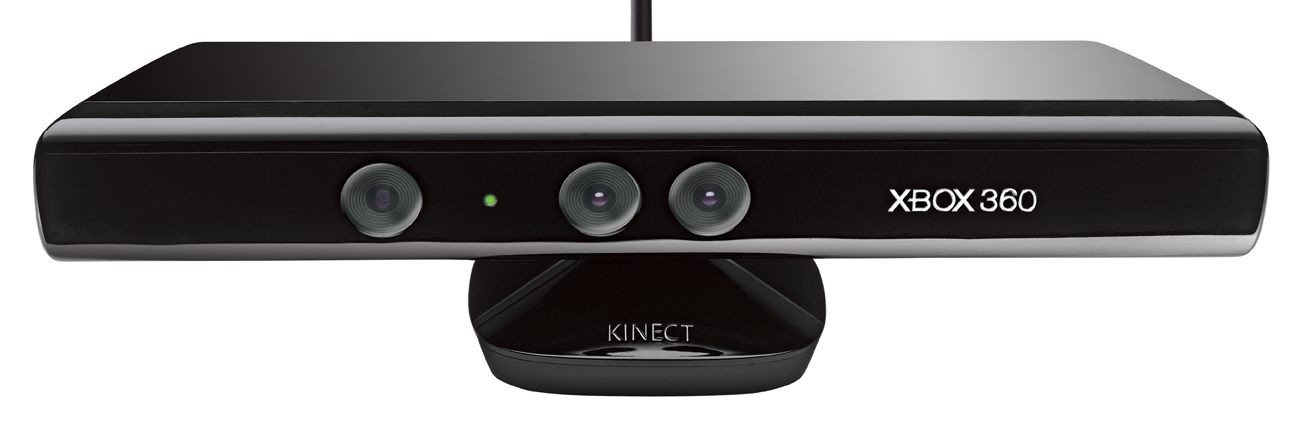
\includegraphics[width=0.75\textwidth]{kinectxbox360}
\caption{Microsoft XBOX 360 Kinect}
\end{figure}

\subsection{Características}
El sensor de Kinect es una barra horizontal de aproximadamente 23 cm (9 pulgadas) conectada a una pequeña base circular con un eje de articulación de rótula, y está diseñado para ser colocado longitudinalmente por encima o por debajo de la pantalla de vídeo.

El dispositivo cuenta con una cámara RGB, un sensor de profundidad, un micrófono de múltiples matrices y un procesador personalizado que ejecuta el software patentado, que proporciona captura de movimiento de todo el cuerpo en 3D, reconocimiento facial y capacidades de reconocimiento de voz.

\begin{figure}[h]
\centering
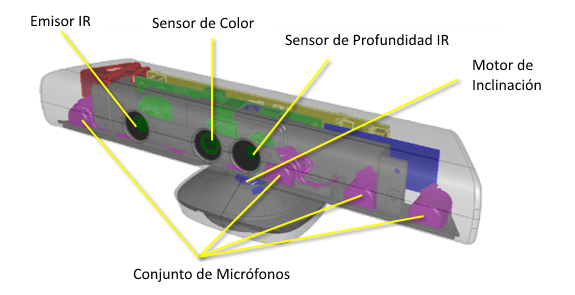
\includegraphics[width=0.75\textwidth]{kinectcomponents}
\caption{Componentes del Kinect}
\end{figure}

El sensor contiene un mecanismo de inclinación motorizado y en caso de usar una PC o un modelo original de Xbox 360, tiene que ser conectado a una toma de corriente a través de un adaptador, ya que la corriente que puede proveerle el cable USB es insuficiente; para el caso del modelo de Xbox 360 S esto no es necesario ya que esta consola cuenta con una toma especialmente diseñada para conectar el Kinect y esto permite proporcionar la corriente necesaria que requiere el dispositivo para funcionar correctamente.

El sensor de profundidad es un proyector de infrarrojos combinado con un sensor CMOS monocromo que permite a Kinect ver la habitación en 3D en cualquier condición de luz ambiental. El rango de detección de la profundidad del sensor es ajustable gracias al software de Kinect capaz de calibrar automáticamente el sensor.

\subsection{Especificaciones Técnicas}
Sus especificaciones \cite{openkinecthardware} \cite{ifixitkinect} más relevantes son:

\begin{itemize}
	\itemsep1pt \parskip1pt \parsep1pt
	\item Cámara / sensor infrarrojo: Microsoft / X853750001 / VCA379C7130 / MT9M001
	\item Rango efectivo (aproximado): 1,2 m – 3,5 m (puede ser menor o mayor, dependiendo de las condiciones ambientales)
	\item Resolución: 640x480 píxeles @ 30 Hz (profundidad de 11 bits: 2048 niveles de sensibilidad)
	\item Cámara RGB: VNA38209015 / MT9M112 / MT9v112
	\item Resolución: 640x480 píxeles @ 30 Hz (VGA de 8 bits)
	\item Emisor / proyector infrarrojo: OG12 / 0956 / D306 / JG05A
	\item Proyector láser de 830 nm.
	\item Potencia de salida: 60\~ mW
\end{itemize}

\subsection{Requerimientos para uso en Robótica}

El Kinect requiere 12 voltios \cite{openkinecthardware} para su funcionamiento (8 V como mínimo); es por ello que, tal como se mencionó anteriormente, la versión para PC cuenta con un adaptador de voltaje adicional, ya que el voltaje proporcionado por la conexión USB es por especificación de 5 voltios.

Es posible encontrar diversos tutoriales en línea \cite{batterypoweredkinect} sobre cómo alimentar al Kinect con la energía necesaria para manejarlo desde un robot autónomo y eliminar la necesidad de utilizar una extensión, asistiendo en su transportabilidad.

\section{Mapas de Entorno}

Uno de los objetivos de un robot autónomo es el de ubicarse a si mismo en el entorno para poder tener la capacidad de interactuar con él, a través de la elaboración de un mapa del mismo. Un mapa es la representación gráfica y métrica, por lo general en un plano, de un territorio o edificio, donde se representan las características físicas del mismo en base a una escala común. En nuestro caso particular, se denominará entonces mapa de entorno a la representación gráfica digitalizada de un entorno perteneciente al interior de un edificio, ya sea un salón, una oficina, un pasillo o demás similares.

\subsection{Tipos de Mapas de Entorno}

La clasificación de un mapa está altamente relacionada con el tipo de uso que pretenda dársele al mismo. \cite{Lee200309} Por ello, podemos clasificarles en una jerarquía según la fortaleza del mapa. En este contexto, la fortaleza del mapa proviene del rango de propiedades geométricas que pueden ser derivadas del mapa; éstas son:

\begin{itemize}
	\itemsep1pt \parskip1pt \parsep1pt
	\item Ubicaciones reconocibles: Consiste en una lista de ubicaciones que pueden ser reconocidas de forma confiable por el robot. No se pueden recuperar relaciones geométricas.
	\item Mapa topológico: Además de contener ubicaciones reconocibles, el mapa guarda cuáles ubicaciones están conectadas por caminos o rutas transitables. Se pueden recuperar las rutas entre ubicaciones ya visitadas.
	\item Mapa topológico métrico: Este término es usado para mapas en el que la información de distancias y ángulos es almacenada junto a las descripciones de las rutas. Se puede recuperar información métrica de las rutas que se han recorrido.
	\item Mapa métrico completo: La ubicación de los objetos se especifica en un sistema de coordenadas fijo. Se puede recuperar información métrica de cualquier objeto en el mapa.
\end{itemize}

Para el propósito de este proyecto, es necesario el uso de un mapa métrico completo, debido a que el robot debe ser capaz de moverse entre espacios libres, evitando obstáculos, teniendo como limitante la ausencia de características distintivas en una ubicación particular (por habitaciones o entornos similares, entornos variables por movimiento de objetos o personas, etc.) y pudiendo contar solamente con las relaciones métricas entre los objetos en el entorno. Podrían utilizarse puntos de referencia, pero sólo como objetos cuya ubicación fuese conocida y que pudiesen ser detectados remotamente (quizás para realizar triangulación).

\subsection{Mapa de Cuadrícula de Ocupación}

Ahora bien, ya se ha mencionado que el mapa debe ser generado a través del propio robot para que éste pueda ser autónomo. Esto introduce una serie de dificultades relacionadas con la exactitud de las mediciones obtenidas por los sensores, tal como se hizo referencia en la sección~\ref{sec:slam}. Una forma de mitigar dichas dificultades tiene que ver con la generación de mapas de cuadrículas de ocupación, que se refiere a una familia de algoritmos probabilísticos cuya idea básica es la de representar un mapa del entorno basado en variables binarias separadas de forma uniforme, donde cada una representa la presencia o ausencia de un obstáculo en esa ubicación del entorno.

\section{Desarrollo Ágil de Proyectos}

En todo proyecto, el objetivo deseado es (o debería ser) el de maximizar la eficiencia y disminuir el costo, ya sea monetario o de tiempo. Para lograr este objetivo se han propuesto diferentes formas de administrar los proyectos, con infinidad de niveles de control, desde prácticamente ningún control en lo absoluto, hasta la microgerencia de las tareas más mínimas posibles.

El desarrollo de un trabajo especial de grado, tesis, o proyecto de grado puede verse, tal como se denominó por último, como un proyecto en si mismo, donde el objetivo es cumplir con los objetivos generales y específicos dentro de un marco de tiempo determinado, por lo que puede aplicarse lo mencionado al inicio para cumplir con los objetivos de la mejor manera posible.

Así pues, en el área de la ingeniería de sistemas y el desarrollo de software, se han empleado igualmente innumerables métodos para llevar a cabo la gerencia de un proyecto; sin que esto pretenda convertirse en un estudio a profundidad de dichos métodos, se nombra a continuación uno de los más populares en la actualidad, junto algunos métodos que emplean su filosofía y cuyo fin no es otro que el de organizar el desarrollo del proyecto y así poder rendir cuentas del mismo.

Las metodologías Ágiles de desarrollo, fueron propuestas en el año 2001 por diversos representantes de múltiples metodologías de desarrollo, tales como SCRUM, Programación Extrema, DSOM, Desarrollo de Software Adaptativo, Crystal y otros, con el fin de encontrar un terreno común que involucrara una alternativa al desarrollo de software pesado y orientado a la documentación.

Su idea consistió en enfocar el proceso de desarrollo en las personas en vez de al proceso en sí, reduciendo la burocracia y los procesos de planificación, documentación y modelado al mínimo posible, a través de principios documentados en un ``manifiesto''.

\subsection{Principios del Desarrollo Ágil}

El manifiesto para el Desarrollo Ágil de Software, indica el enfoque a seguir por esta metodología. Sus valores principales son los siguientes:

\begin{itemize}
	\itemsep1pt \parskip1pt \parsep1pt
	\item Individuos e interacciones sobre procesos y herramientas
	\item Software funcionando sobre documentación extensiva
	\item Colaboración con el cliente sobre negociación contractual
	\item Respuesta ante el cambio sobre seguir un plan
\end{itemize}

En las propias palabras del manifiesto: ``Esto es, aunque valoramos los elementos de la derecha, valoramos más los de la izquierda''.\cite{beck2001manifiesto}

Los principios producto de estos valores son:\cite{beck2001principios}

\begin{itemize}
	\itemsep1pt \parskip1pt \parsep1pt
	\item Nuestra mayor prioridad es satisfacer al cliente mediante la entrega temprana y continua de software con valor.
	\item Aceptamos que los requisitos cambien, incluso en etapas tardías del desarrollo. Los procesos Ágiles aprovechan el cambio para proporcionar ventaja competitiva al	cliente.
	\item Entregamos software funcional frecuentemente, entre dos semanas y dos meses, con preferencia al periodo de tiempo más corto posible.
	\item Los responsables de negocio y los desarrolladores	trabajamos juntos de forma cotidiana durante todo el proyecto.
	\item Los proyectos se desarrollan en torno a individuos motivados. Hay que darles el entorno y el apoyo que necesitan, y confiarles la ejecución del trabajo.
	\item El método más eficiente y efectivo de comunicar información al equipo de desarrollo y entre sus miembros es la conversación cara a cara.
	\item El software funcionando es la medida principal de	progreso.
	\item Los procesos Ágiles promueven el desarrollo sostenible. Los promotores, desarrolladores y usuarios
	debemos ser capaces de mantener un ritmo constante de forma indefinida.
	\item La atención continua a la excelencia técnica y al	buen diseño mejora la Agilidad.
	\item La simplicidad, o el arte de maximizar la cantidad de	trabajo no realizado, es esencial.
	\item Las mejores arquitecturas, requisitos y diseños emergen de equipos auto-organizados.
	\item A intervalos regulares el equipo reflexiona sobre	cómo ser más efectivo para a continuación ajustar y perfeccionar su comportamiento en consecuencia.
\end{itemize}

\section{Personal Extreme Programming}
La programación extrema o \textit{eXtreme Programming} (XP) es una metodología de desarrollo de la ingeniería de software formulada por Kent Beck, autor del primer libro sobre la materia, \textit{Extreme Programming Explained: Embrace Change} (1999). Es el más destacado de los procesos ágiles de desarrollo de software. Al igual que éstos, la programación extrema se diferencia de las metodologías tradicionales principalmente en que pone más énfasis en la adaptabilidad que en la previsibilidad.

Los defensores de XP consideran que los cambios de requisitos sobre la marcha son un aspecto natural, inevitable e incluso deseable del desarrollo de proyectos. Creen que ser capaz de adaptarse a los cambios de requisitos en cualquier punto de la vida del proyecto es una aproximación mejor y más realista que intentar definir todos los requisitos al comienzo del proyecto e invertir esfuerzos después en controlar los cambios en los requisitos.

Se puede considerar la programación extrema como la adopción de las mejores metodologías de desarrollo de acuerdo a lo que se pretende llevar a cabo con el proyecto, y aplicarlo de manera dinámica durante el ciclo de vida del software.

\subsection{Características}
Las características fundamentales del método son:

\begin{itemize}
	\itemsep1pt \parskip1pt \parsep1pt
	\item Desarrollo iterativo e incremental: pequeñas mejoras, unas tras otras.
	\item Pruebas unitarias continuas, frecuentemente repetidas y automatizadas, incluyendo pruebas de regresión. Se aconseja escribir el código de la prueba antes de la codificación. Véase, por ejemplo, las herramientas de prueba JUnit orientada a Java, DUnit orientada a Delphi, NUnit para la plataforma.NET o PHPUnit para PHP. Estas tres últimas inspiradas en JUnit, la cual, a su vez, se inspiró en SUnit, el primer framework orientado a realizar tests, realizado para el lenguaje de programación Smalltalk.
	\item Programación en parejas: se recomienda que las tareas de desarrollo se lleven a cabo por dos personas en un mismo puesto. La mayor calidad del código escrito de esta manera -el código es revisado y discutido mientras se escribe- es más importante que la posible pérdida de productividad inmediata. En este sentido, la modalidad personal difiere por razones obvias; sin embargo, las demás características son perfectamente aplicables.
	\item Frecuente integración del equipo de programación con el cliente o usuario. Se recomienda que un representante del cliente trabaje junto al equipo de desarrollo.
	\item Corrección de todos los errores antes de añadir nueva funcionalidad. Hacer entregas frecuentes.
	\item Refactorización del código, es decir, reescribir ciertas partes del código para aumentar su legibilidad y mantenibilidad pero sin modificar su comportamiento. Las pruebas han de garantizar que en la refactorización no se ha introducido ningún fallo.
	\item Propiedad del código compartida: en vez de dividir la responsabilidad en el desarrollo de cada módulo en grupos de trabajo distintos, este método promueve el que todo el personal pueda corregir y extender cualquier parte del proyecto. Las frecuentes pruebas de regresión garantizan que los posibles errores serán detectados.
	\item Simplicidad en el código: es la mejor manera de que las cosas funcionen. Cuando todo funcione se podrá añadir funcionalidad si es necesario. La programación extrema apuesta que es más sencillo hacer algo simple y tener un poco de trabajo extra para cambiarlo si se requiere, que realizar algo complicado y quizás nunca utilizarlo.
\end{itemize}

La simplicidad y la comunicación son extraordinariamente complementarias. Con más comunicación resulta más fácil identificar qué se debe y qué no se debe hacer. Cuanto más simple es el sistema, menos tendrá que comunicar sobre éste, lo que lleva a una comunicación más completa, especialmente si se puede reducir el equipo de programadores.

\section{Kanban}

Kanban, del japonés \begin{CJK*}{UTF8}{gbsn}かんばん\end{CJK*}(\begin{CJK*}{UTF8}{gbsn}看板\end{CJK*}), que es literalmente ``letrero'' o ``cartelera'', es un sistema de programación para la producción \textit{Lean} y justo-a-tiempo.

Kanban se basa en una idea muy simple: el trabajo en curso (\textit{Work In Progress}, WIP) debería limitarse, y sólo deberíamos empezar con algo nuevo cuando un bloque de trabajo anterior haya sido entregado o ha pasado a otra función posterior de la cadena. El Kanban (o tarjeta señalizadora) implica que se genera una señal visual para indicar que hay nuevos bloques de trabajo que pueden ser comenzados porque el trabajo en curso actual no alcanza el máximo acordado.

Kanban usa un mecanismo de control visual para hacer seguimiento del trabajo conforme este viaja a través del flujo de valor. Típicamente, se usa un panel o pizarra con notas adhesivas o un panel electrónico de tarjetas. Las mejores prácticas apuntan probablemente al uso de ambos.

Las metodologías Ágiles han obtenido buenos resultados proporcionando transparencia respecto al trabajo en curso y completado, así como en el reporte de métricas como la velocidad (cantidad de trabajo realizada en una iteración). Kanban sin embargo va un paso más allá y proporciona transparencia al proceso y su flujo. Kanban expone los cuellos de botella, colas, variabilidad y desperdicios. Todas las cosas que impactan al rendimiento de la organización en términos de la cantidad de trabajo entregado y el ciclo de tiempo requerido para entregarlo. Kanban proporciona a los miembros del equipo y a las partes interesadas visibilidad sobre los efectos de sus acciones (o falta de acción). De esta forma, los casos de estudios preliminares están demostrando que Kanban cambia el comportamiento y motiva a una mayor colaboración en el trabajo. La visibilidad de los cuellos de botella, desperdicios y variabilidades y su impacto también promueve la discusión sobre la posibles mejoras, y los equipos comienzan rápidamente a implementar mejoras en su proceso.\cite{Skarin201003}

\subsection{Trello}

Trello es una plataforma de software que utiliza el paradigma Kanban para el manejo de proyectos. Iniciado en el año 2011 por la compañía Fog Creek Software y caracterizado como software de productividad, este utiliza un sistema de tableros, listas y tarjetas para llevar el control de múltiples tipos de proyecto, sin estar limitado a proyectos de desarrollo de software, por lo cual es altamente versátil. Las tarjetas aceptan comentarios, archivos adjuntos, votos, fechas de entrega y listas de verificación.

Para este proyecto, se abrió un tablero en Trello accesible desde la dirección \url{https://trello.com/b/yIMdcTCR/tesis-ros-kinect}, cuyas listas representan un híbrido entre las disponibles en PXP y Kanban, de la siguiente manera:

\begin{itemize}
	\itemsep1pt \parskip1pt \parsep1pt
	\item Pendientes: Tareas que están por ser ejecutadas.
	\item Actuales: Tareas que están siendo ejecutadas actualmente.
	\item Entregadas: Tareas que están marcadas como realizadas, pero que no han sido verificadas aún.
	\item Rechazadas: Tareas que, habiendo sido entregadas, presentan alguna falla o requieren algún cambio, por lo cual se colocan en esta lista para ser revisadas.
	\item Listas: Tareas que han sido verificadas y aceptadas.
	\item Ideas: Tarjetas que representan ideas aplicar, o tareas que no pueden pasar a la lista ``Pendientes'' por no haber recursos disponibles para ellas.
\end{itemize}

\begin{figure}[ht]
\centering
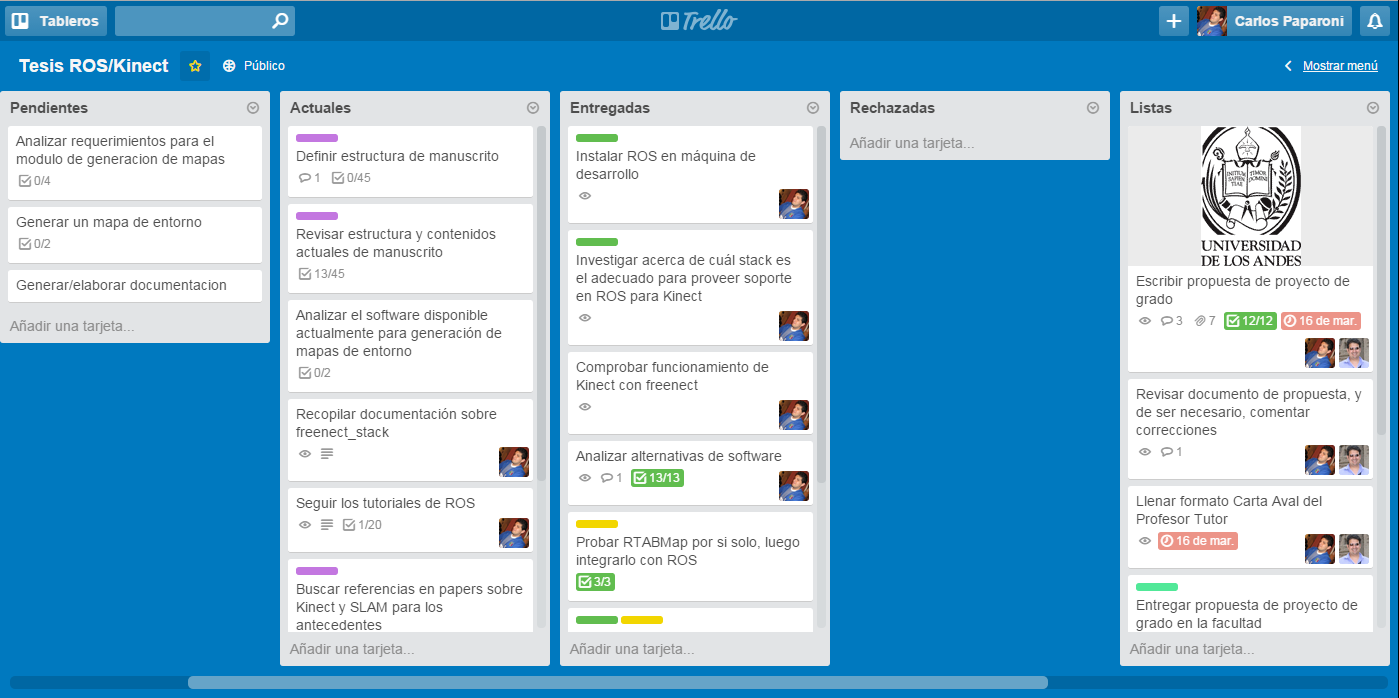
\includegraphics[width=1.00\textwidth]{trelloprojectwindow}
\caption{Tablero en Trello para el proyecto de grado}
\end{figure}

\subsubsection{Uso}

Cada tarea a realizar se coloca como una tarjeta en la lista correspondiente a ``Pendientes'' o ``Ideas'' según sea el caso, y una vez estén disponibles los recursos para tomarla (siendo estos recursos tiempo, o disponibilidad de la o las personas involucradas) se pasa dicha tarjeta, mediante arrastrar y colocar, a la lista de ``Actuales''. Esto permite ver el flujo de trabajo, tal como se mencionaba anteriormente, y permite saber el estado actual del proyecto si la tabla se mantiene actualizada.

Una vez terminada la tarea, se coloca en la lista ``Entregadas'', para su revisión (en el caso de este proyecto, el cliente del mismo viene a ser el profesor tutor, quien es la persona que puede verificar que se haya llevado a cabo satisfactoriamente o no). En caso que la tarea esté correcta, se puede pasar a la lista ``Listas'', lo cual marca la finalización de la tarea, y la liberación de los recursos empleados para tomar nuevas tareas disponibles. En caso de observar algún error, la tarea pasa a la lista ``Rechazadas'', para su revisión y corrección.
 % Marco teórico

\chapter{Software de Control Robótico}

Este capítulo pretende ahondar en las características de las plataformas o software de control robótico, comenzando por su definición, la exposición de las características más comunes, los criterios bajo los cuales se selecciona una lista de posibles plataformas para el desarrollo del proyecto y finalmente, la justificación de la plataforma de software escogida.

\section{Definición}

Por lo general, cuando se piensa en robótica el enfoque se realiza sobre los componentes de hardware: actuadores, motores, sensores, etc., y se piensa muy poco sobre el software de control que se utilizará.

Podemos comenzar por definir dicho software como el conjunto de módulos o programas que se encarga indicarle al hardware del robot qué tareas o funciones debe realizar. Dichas funciones son altamente variadas y van desde el control de los actuadores o sensores hasta el manejo de algoritmos de navegación autónoma o reconocimiento del terreno.

Definir una plataforma común de software para múltiples robots es un reto porque, a menos que sean robots construidos en masa y con un propósito igualmente común, normalmente no hay dos robots iguales, o con la misma estructura y/o componentes. No obstante, la forma de crear una aplicación para un robot no es distinta de la empleada para crear cualquier otro tipo de aplicación: un desarrollador escribe la aplicación en determinado lenguaje, lo compila enlazado con las bibliotecas adecuadas para ser ejecutado en determinado sistema operativo y por último, ejecutarlo en el computador que controla al robot.

\subsection{Software de Robots}

Si bien el proceso de desarrollo de software para robots posee muchas características comunes con el desarrollo de una aplicación común, éstos cuentan con requerimientos específicos que deben ser tomados en cuenta. Desarrollar software para robots móviles es una tarea compleja, ya que un robot es un sistema complejo en si mismo y además este proceso suele ser más exigente que la creación de una aplicación ``estándar'' como manejadores de bases de datos, \textit{suites} ofimáticas, etc. Los siguientes son algunos condicionantes propios, que diferencian el desarrollo de software robótico de otros ámbitos:

\begin{enumerate}
	\itemsep1pt \parskip1pt \parsep1pt
	\item A diferencia de una aplicación estándar, una aplicación robótica está directamente enlazada a la realidad física, donde dicho enlace es llevado a cabo a través de sensores y actuadores, donde los primeros obtienen información del entorno y los segundos la modifican. Por tanto, el programa debe poder responder a cualquier cambio en el entorno de forma ágil, para así poder enviar ajustes a los actuadores rápidamente. Esto obliga a que la actuación del software entre en la categoría de tiempo real, como mínimo \textit{soft} o blando, si no estricto.

	\item Por lo general, un robot debe realizar múltiples tareas a la vez: monitorear sensores, actualizar la interfaz gráfica con el usuario, enviar órdenes a los actuadores, comunicar datos a otros procesos, procesar datos, etc., por lo cual se requiere concurrencia y esto añade complejidad, en mayor o menor grado.

	\item Si bien esto no es imprescindible (en especial en robots autónomos), el software que es ejecutado en el robot debe actualizar constantemente la interfaz gráfica con el usuario, ya que es una herramienta muy útil para realizar depuración de datos y comportamiento y para visualizar en tiempo de ejecución, las estructuras y variables internas, tales como representaciones del mundo, mapas, estados, etc.

	\item Siguiendo los actuales esquemas de desarrollo de software, el software de robots es cada vez más distribuido. Es usual que las aplicaciones de robots tengan que establecer alguna comunicación con otros procesos ejecutándose en la misma máquina o en una diferente. La distribución ofrece posibilidades ventajosas como ubicar la carga computacional en nodos con mayor capacidad o la visualización remota; y en sistemas multirrobot, hace posible la integración sensorial, la centralización y la coordinación.

	\item La diversidad que existe, tanto en hardware como software, hace más compleja la tarea de programación. En cuanto al hardware, cada día se hace mayor la gran diversidad de dispositivos sensoriales y de actuación, y por lo tanto de interfaces; esto obliga al programador a dominarlos para acceder a ellos desde las aplicaciones. Por otro lado, mientras que en muchos campos de la informática sí hay bibliotecas que un programador puede emplear para construir su propio programa, en el software de robots no hay un marco homogéneo ni hay estándares que propicien la reutilización de código y la integración. En robótica cada aplicación prácticamente ha de construirse desde cero para cada robot concreto.

	\item Ya que el campo que estudia el comportamiento de robots, para dividirlo en unidades básicas sigue siendo materia de investigación, no existe una guía universalmente admitida sobre la forma de organizar el código de las aplicaciones de robots para que sean escalables y reutilizables. Cada desarrollador escribe su aplicación combinando \textit{ad-hoc} los bloques de código que puedan existir en su entorno.
\end{enumerate}

\subsection{Plataformas de Software}

De la misma forma como los dispositivos electromecánicos -mejor conocidos como robots- que pretenden controlar, el software escrito para ellos presenta, con el pasar del tiempo, cada vez más complejidad y ofrecen mayor funcionalidad. Para ayudar con ambos aspectos, se ha ido implantando \textit{middleware} que simplifica el desarrollo de nuevas aplicaciones en esas áreas, proporcionando contextos nítidos, estructuras de datos predefinidas, bloques muy depurados de código de uso frecuente, protocolos estándar de comunicaciones, mecanismos de sincronización, etc. De forma paralela, a medida que el desarrollo de software para robots móviles ha ido madurando también han ido apareciendo diferentes plataformas \textit{middleware}.

Actualmente, los fabricantes más avanzados incluyen plataformas de desarrollo para simplificar a los usuarios la programación de sus robots. Por ejemplo, ActivMedia ofrece la plataforma ARIA para sus robots Pioneer, PeopleBot, etc.; iRobot ofrecía Mobility para sus B14 y B21; Evolution Robotics vende su plataforma ERSP; y Sony ofrece OPEN-R para sus Aibo.

De igual forma, muchos grupos de investigación han creado sus propias plataformas de desarrollo. Varios ejemplos son la suite de navegación CARMEN de Carnegie Mellon University, OROCOS, Player/Stage/Gazebo (PSG), Miro, JDE, MARIE, etc..

El objetivo fundamental de estas plataformas es hacer más sencilla la creación de aplicaciones para robots, a través de las siguientes características comunes: uniformar y simplificar el acceso al hardware, ofrecer una arquitectura de software concreta y proporcionar un conjunto de bibliotecas o módulos con funciones de uso común en robótica que el cliente puede reutilizar para programar sus propias aplicaciones.

Este objetivo se intenta lograr mediante las siguientes acciones: \cite{canas06programacion}

\begin{itemize}
	\itemsep1pt \parskip1pt \parsep1pt
	\item Abstracción del Hardware:

	El sistema operativo provee acceso a sensores y actuadores, aunque lo hace de forma más definida y compleja, totalmente opuesto a como lo hacen las plataformas. Un ejemplo de esto es el siguiente: si se dispone de un robot Pioneer equipado con un sensor láser SICK, la aplicación puede acceder a sus medidas a través de las funciones de la plataforma ARIA o pedirlas y recogerlas directamente a través del puerto serie. Utilizando ARIA basta invocar un método sobre cierto objeto de una clase y la plataforma se encargará de mantener actualizadas las variables con las lecturas. Utilizando sólo el sistema operativo, la aplicación debe solicitar y recoger periódicamente las lecturas al sensor láser a través del puerto serie, y debe conocer el protocolo del dispositivo para componer y analizar correctamente esos mensajes de bajo nivel.

	De la misma forma se ofrece el acceso abstracto para los actuadores. Por ejemplo, en vez de ofrecer comandos de velocidad para cada una de las dos ruedas motrices de un robot Pioneer, la plataforma Miro ofrece una sencilla interfaz de V-W (velocidad de tracción y de giro) para la actuación motriz, la cual se encarga de hacer las transformaciones oportunas, de enviar a cada rueda las consignas necesarias para que el robot consiga esas velocidades comandadas de tracción y de giro.

	En virtud que hay gran heterogeneidad en cuanto al hardware dentro de la robótica, un primer paso bastante importante para llevar a cabo la reutilización de software es la de homogeneizar el acceso al hardware; esta característica está presente en varias plataformas, aunque cada una lo hace a su manera. En la plataforma ERSP de Evolution Robotics el acceso al bajo nivel recibe el nombre de \textit{Hardware Abstraction Layer} (HAL), y en Miro, \textit{Service Layer}. En OPEN-R, en Mobility y en ARIA la API de acceso a los sensores y actuadores viene dada por los métodos de un conjunto objetos. En JDE y en PSG el acceso abstracto al hardware lo marca un protocolo entre las aplicaciones y los servidores.

	\item Arquitectura de software:

	La arquitectura de software defina la manera como se accede a los sensores, motores o funcionalidades por parte del código de la aplicación. Para hacerlo, se pueden realizar llamados a funciones, invocar métodos, enviar mensajes, leer variables, entre otros. Algunos ejemplos de esto los proveen CARMEN al usar interfaces funcionales, Miro al realizar invocación de métodos de objetos distribuidos, TCA al pasar mensajes entre módulos y JDE al leer y escribir variables y activar procesos.

	Así mismo, el software escrito para la plataforma de software particular, también toma la misma arquitectura. Mencionando los mismos ejemplos del párrafo anterior, en CARMEN se puede plantear el software como un conjunto de interfaces, en Miro, como una colección de métodos, en TCA, como un conjunto de módulos que pasan mensajes entre sí a través de la red, etc. Esto puede restringir en mayor o menor grado la forma como se realiza el software, de forma cerrada (muy restrictiva) o abierta (restricción en mínima cantidad.)

	A medida que se avanza en complejidad, cada plataforma utiliza mecanismos concretos para poder distribuirse en múltiples unidades de forma concurrente. El mecanismo multitarea que ofrece la plataforma envuelve y simplifica la interfaz del \textit{kernel} subyacente para la multiprogramación, en la cual se apoyan siempre. Al igual que ocurre con la interfaz abstracta de acceso al hardware, la interfaz de multitarea abstracta facilita la portabilidad.

	\item Funcionalidades de uso común:

	Permite la reutilización (de forma íntegra o por partes) de funcionalidades básicas como filtros de color y complejas como algoritmos de control o técnicas de percepción, tales como: localización, navegación local segura, navegación global, seguimiento de personas, habilidades sociales, construcción de mapas, etc. Esto reduce la repetición de código y por ende, de trabajo y de esfuerzo de programación. Por otro lado, el código ya provisto es extensamente probado en búsqueda de errores, lo cual se traduce en menor cantidad de errores en el programa completo, permitiéndole al desarrollador concentrarse en escribir su aplicación y no en detalles de bajo nivel.
	Esto se lleva a cabo dependiendo de la arquitectura de software y del encapsulamiento realizado por ella. Dependiendo del modelo de negocios de los fabricantes, estas funcionalidades pueden venir incluidas con su aplicación, o venderse por separado.

	\item Arquitectura cognitiva:

	La arquitectura cognitiva de un robot se refiere a la forma como se organizan sus capacidades sensoriales y de actuación para generar un conjunto de comportamientos: para comportamientos simples cualquier organización puede resultar válida, no así para comportamientos complejos, ya que con una mala organización la complejidad puede tornarse inmanejable.

	Dividir el comportamiento artificial en unidades reutilizables es una cuestión muy complicada. Se considera que hasta el momento es muy pronto pretender buscar estándares en esta área y se recomienda sólo enfocar la estandarización de forma exclusiva al acceso a los sensores y actuadores.

	Existen múltiples relaciones entre las arquitecturas de software y cognitivas: las cognitivas se materializan en alguna arquitectura de software, por tanto, los comportamientos que son generados siguiendo un determinado paradigma terminan siendo implementados con algún programa concreto.

	Entre las propuestas cognitivas más fiables contamos con arquitecturas de software deliberativas, híbridas, basadas en comportamientos, etc, con el objetivo de favorecer la escalabilidad de la plataforma.

	No todas las plataformas están basadas en un modelo cognitivo; algunas combinan más adecuadamente con determinadas escuelas cognitivas, dependiendo del sistema en el que esté: los deliberativos clásicos van de la mano con la programación lógica, descompuestos funcionalmente en bibliotecas y manteniendo un solo flujo de control iterativo, mientras que los sistemas basados en comportamientos van mejor con la programación concurrente, con varios módulos ejecutados en paralelo.

	\item Plataformas de software libre:

	La intención tras liberar el código fuente bajo licencias de software libre por parte de los grupos de investigación, es la de contribuir con el libre intercambio de información en el área, ayudando al avance de la disciplina robótica. Unos ejemplos de estos (algunos de los cuales serán mencionados más adelante) son los siguientes:

	\begin{itemize}
		\item ARIA: \textit{Advanced Robot Interface for Applications} o ARIA es desarrollada y mantenida por ActivMedia Robotics específicamente para sus robots, pero liberada bajo licencia GPL. Está diseñado como cliente/servidor y su entorno de programación es orientado a objetos (aunque sus objetos no son distribuidos sino ubicados en la máquina conectada físicamente al robot) e incluye soporte para comunicaciones por red y programación multitarea. A diferencia de CARMEN, sus aplicaciones deben de escribirse en C++, aunque provee soporte en Linux y Windows de 32 bits.

		Para acceder al hardware se provee una colección de clases que conforman una API (\textit{Application Programming Interface} -- Interfaz de Programación de Aplicación), tales como ArRobot, Packet Receiver, Packet Sender, ArRangeDevices, ArSonarDevice, ArSick, ArNetworking, ArPeriodicTask o ArThreads, entre otras. Estas son incluidas como comportamientos básicos integrados en la plataforma; otros comportamientos tales como la construcción de mapas, navegación, localización o la identificación de objetos por color y su seguimiento se venden por separado.

		\item Miro: es una plataforma orientada a objetos (distribuidos) basada en la arquitectura/estándar CORBA (\textit{Common Object Request Broker Architecture}), desarrollada en la Universidad de Ulm en Alemania y publicada bajo la licencia LGPLv2. Miro no impone ninguna restricción en el lenguaje de programación utilizado, aunque está escrito enteramente en C++.  Consta de tres niveles: una capa de dispositivos, que proporciona interfaces en forma de objetos para actuadores y sensores, una capa de servicios, que provee la descripción de las interfaces anteriores haciéndolas accesibles remotamente, y el entorno de clases, que contiene herramientas para visualización, generación de históricos así como módulos comunes y ya mencionados previamente, como construcción de mapas, generación de comportamientos o planificación de caminos.

		\item Player/Stage/Gazebo (PSG): creada inicialmente en la Universidad de South California; comprende los simuladores Stage y Gazebo y el servidor Player al que se conectan las aplicaciones mediante una arquitectura cliente/servidor para recoger datos sensoriales o comandar órdenes a los actuadores. Esto le proporciona una independencia de lenguaje y mínimas restricciones de arquitectura. Es una plataforma muy completa debido a los simuladores que incorpora y a que provee soporte a gran variedad de robots; sumado a esto, cuenta con una creciente y muy activa comunidad de desarrolladores, que añade nuevas capacidades y amplía el hardware soportado. Su forma de funcionamiento es basada en archivos al estilo de Unix, representando mediante estos a los sensores y actuadores, proveyendo las cinco operaciones básicas sobre los mismos: apertura, lectura, escritura, configuración y cierre. De igual manera, los dispositivos se organizan por categorías, abstrayéndolos mediante interfaces comunes.
	\end{itemize}
\end{itemize}

Por lo visto anteriormente, y dadas sus ventajas, podemos considerar que la mejor opción para unificar el desarrollo de plataformas robóticas en el aspecto de software es hacerlo a través de (\textit{frameworks}) o plataformas de software.

\section{Criterios de Selección}

Antes de mencionar las plataformas consideradas para el desarrollo de este proyecto, es muy importante destacar la forma éstas como serán discriminadas con la finalidad de seleccionar la más adecuada para el uso futuro en LaSDAI.

En primer lugar, y atendiendo a las diversas ventajas que esto implica, se enfoca como uno de los principales requisitos indispensables que la plataforma de software esté desarrollada o posea licencias de Software Libre, ya que esto facilita cualquier desarrollo futuro que desee realizarse en él. La existencia o ausencia de licencias de Software Libre basta como criterio en si mismo.

Después, se espera que dicha plataforma cuente con soporte actual de la comunidad: es decir, que existan grupos de usuarios en foros y/o listas de correo que estén activas y que respondan a dudas de los usuarios. También se toma en cuenta que exista soporte por parte del equipo de desarrolladores a cargo de la plataforma y que ésta sea actualizada regularmente. Esto es sumamente importante ya que hace más factible que nuevos desarrolladores puedan obtener respuesta a sus consultas o inconvenientes y que en caso de existir estos últimos, se pueda llegar a corregirlos. Para evaluar este criterio, se toman en cuenta la cantidad de grupos disponibles para consulta, de preferencia a través de foros de ayuda y la última fecha de actualización de la plataforma de software como tal; mientras más reciente, mejor.

Luego, se tiene como requerimiento altamente deseable (mas no excluyente), que dicha plataforma soporte los lenguajes de programación en uso actualmente por LaSDAI, o cuyo uso pueda ser deseable en un futuro no muy lejano. Este criterio se da por existente si la plataforma soporta al menos uno de los lenguajes mencionados.

Además, en virtud que este proyecto está basado en el uso del Kinect como sensor para generación de mapas de entorno, no es de extrañar que este sea un requerimiento con alto peso, ya que al contar con soporte ya existente, hace más sencilla la tarea de llevar a cabo la generación de mapas en un robot móvil. Si la plataforma cuenta con al menos un módulo soportado actualmente por algún desarrollador o grupo de desarrolladores, se coloca este criterio como afirmativo.

Por último, aunque vinculado al segundo requisito, se desea que la plataforma de software a escoger, posea documentación amplia y frecuentemente actualizada, porque sólo un programador sabe cuán difícil es desarrollar en un nuevo entorno sin poder contar con documentación o referencias adecuadas. Este criterio basa su existencia o ausencia en una evaluación propia y por tanto, subjetiva de la documentación, ya que establecer una serie de reglas para la evaluación de este criterio, es una materia de estudio en si mismo.

\subsection{Evaluación de Criterios}

Para llevar a cabo la evaluación de cada plataforma, se procedió de la siguiente manera:

Por cada uno de los elementos en la lista de plataformas (Tabla \ref{table:platcons}), se realizó una búsqueda no-exhaustiva en los motores de búsqueda correspondientes a Google Web (\url{https://google.com/}) y Google Académico (\url{https://scholar.google.co.ve/}), buscando a su vez características en la lista de criterios para cada uno, evaluándose en cuanto a existencia o ausencia de cada parámetro, o en el caso de criterios que podían ser parciales, colocando la simbología correspondiente, tal como se detalló en la sección pasada.

\section{Plataformas de Software Consideradas}

\begin{table}[H]
\begin{adjustbox}{max width=\textwidth}
\begin{threeparttable}
\centering
\begin{tabular}{@{}lccccc@{}}
\toprule
\multicolumn{1}{c}{{\bf \begin{tabular}[c]{@{}c@{}}Plataforma de\\ Software\end{tabular}}} & {\bf \begin{tabular}[c]{@{}c@{}}Software\\ Libre\end{tabular}} & {\bf \begin{tabular}[c]{@{}c@{}}Soportado por\\ la Comunidad\end{tabular}} & {\bf \begin{tabular}[c]{@{}c@{}}Soporte\\ C / C++ / Python\end{tabular}} & {\bf \begin{tabular}[c]{@{}c@{}}Soporte\\ Kinect\end{tabular}} & {\bf \begin{tabular}[c]{@{}c@{}}Documentación\\ Actualizada\end{tabular}} \\ \midrule
CARMEN                                           & \cmark                             & \xmark                                   & \cmark                                  & \xmark                             & O                                     \\
Microsoft Robotics Developer Studio                            & \xmark                             & \xmark                                   & \xmark                                  & \cmark                             & \cmark                                  \\
MOOS                                            & \cmark                             & \text{\sffamily O}                             & \cmark                                  & \xmark                             & \text{\sffamily O}                            \\
OpenRDK                                          & \cmark                             & \text{\sffamily O}                             & \cmark                                  & \xmark                             & \cmark                                  \\
OpenRTM-aist                                        & \cmark                             & \cmark                                   & \cmark                                  & \cmark                             & \cmark                                  \\
ORCA                                            & \cmark                             & \xmark                                   & \cmark                                  & \xmark                             & \cmark                                  \\
Player                                           & \cmark                             & \text{\sffamily O}                             & \cmark                                  & \cmark                             & \cmark                                  \\
Robot Construction Kit (RoCK)                               & \cmark                             & \text{\sffamily O}                             & \text{\sffamily O}                            & \cmark                             & \cmark                                  \\
Robot Operating System (ROS)                                & \cmark                             & \cmark                                   & \cmark                                  & \cmark                             & \cmark                                  \\
Yet Another Robot Platform (YARP)                             & \cmark                             & \text{\sffamily O}                             & \cmark                                  & \text{\sffamily O}                       & \cmark                                  \\ \bottomrule
\end{tabular}
\begin{tablenotes}
\item Leyenda: \cmark = sí, \text{\sffamily O} = parcial, \xmark = no
\end{tablenotes}
\end{threeparttable}
\end{adjustbox}
\caption{Plataformas de Software consideradas}\label{table:platcons}
\end{table}

\section{Plataforma de Software Seleccionada}

Dada la popularidad, la facilidad de uso e independencia de lenguajes del sistema de comunicación interprocesos, la fácil integración de una amplia gama de herramientas como las de visualización de los datos de movimiento y sensores del robot, implementación de los algoritmos de planificación de ruta y de percepción y controladores de bajo nivel para sensores comúnmente utilizados y las herramientas de administración que permiten el monitoreo y la inspección de mensajes, hacen que ROS sea el candidato perfecto para el uso en proyectos en el área de robótica móvil.

Por último pero no por ello menos importante, ROS cuenta con amplia documentación \cite{answersros} para cualquier nivel de usuario, desde principiante hasta experto, por lo que cualquier nuevo desarrollo puede efectuarse con una curva de aprendizaje leve, desde el punto de vista coloquial de esta frase. De igual forma, también cuenta con múltiples foros activos donde los mismos usuarios interactúan para consultar y resolver dudas. % Software de Control Robótico

\chapter{ROS}

En este capítulo se desea profundizar en la definición de ROS (Robot Operating System) como plataforma de software seleccionada para el desarrollo de este proyecto de grado. Asimismo, se describen sus características principales, la arquitectura de software que utiliza, la instalación del mismo en el entorno de desarrollo a utilizar, y los módulos en los cuales se apoya este proyecto para llevar a cabo la generación de mapas de entorno.

\section{Definición}

\textit{Robot Operating System} (Sistema Operativo de/para Robot) o sencillamente ROS, es, tal como su nombre implica, un sistema operativo para robots, de forma similar a los sistemas operativos para computadores de escritorio o servidores. Desarrollado y mantenido por la empresa Willow Garage, es una colección de herramientas, librerías y convenciones que buscan simplificar la tarea de crear comportamientos de robot robustos y complejos a lo largo de una amplia variedad de plataformas robóticas.

La justificación de porqué hacer esto es porque decididamente, crear software robótico de propósito general y verdaderamente robusto es difícil, ya que si bien para un ser humano algunos problemas son triviales, no lo son en lo absoluto al momento de tomar en cuenta las grandes variaciones entre instancias de tareas y entornos. Lidiar con estas variaciones es tan complicado que ningún individuo, laboratorio o institución pudiera esperar llevarlo a cabo por su propia cuenta.

Por ello, ROS fue construido desde cero con el fin de alentar el desarrollo de software robótico de forma colaborativa. Un ejemplo de esto es que, un laboratorio podría tener expertos en cartografía o mapeado de interiores y podría contribuir un sistema de excelente calidad para la producción de mapas. Otro grupo podría tener expertos en el uso de mapas para navegar, y otro grupo podría haber descubierto un enfoque de visión por computador que funciona bien para el reconocimiento de objetos pequeños entre el desorden. ROS fue diseñado específicamente para grupos como éstos para colaborar y construir sobre el trabajo del otro. \cite{aboutros}

Además, ROS es Software Libre y está distribuido bajo la licencia BSD, permitiendo el desarrollo de proyectos comerciales y no-comerciales. Una característica importante en cuanto a la arquitectura (que se detallará más adelante) es que ROS funciona a través de comunicación entre procesos, sin requerir que los módulos sean enlazados dentro del mismo ejecutable, por lo que cualquier sistema construido usando ROS como base puede tener control detallado sobre las licencias de software que utilicen sus módulos, ya sean GPL, BSD o cualquier otra hasta propietaria. \cite{quigley2009ros}

\section{Características Principales}

Se pueden comentar las siguientes:

\begin{description}
	\item[Comunicación entre pares:] los sistemas robóticos complejos con múltiples enlaces podrían tener varios computadores de a bordo (para realizar tareas paralelas) conectados a través de una red. La ejecución de un maestro central podría dar lugar a la congestión severa en un enlace determinado. Usando una comunicación peer-to-peer o entre pares evitaría este problema. En ROS, una arquitectura peer-to-peer acoplado a un sistema de memoria intermedia o buffer y un sistema de búsqueda (un servicio de nombres llamado ``maestro'' en ROS), le permite a cada componente dialogar directamente con cualquier otro, de forma sincrónica o asincrónica como sea necesario.

	\item[Gratuito y de código abierto:] Ser una plataforma de código abierto ofrece la reutilización de funciones ya existentes proporcionadas por muchos otros usuarios de ROS. Su código se suministra en repositorios como stacks, o ``pilas''. Otras personas han desarrollado capacidades sorprendentes para los robots que han sido ``de código abierto'' y son relativamente fáciles de añadir de forma incremental utilizando el entorno de desarrollo de ROS.

	\item[Delgado:] Para combatir el desarrollo de algoritmos que se ``enredan'' o vinculan en un grado mayor o menor con el sistema operativo del robot y, por tanto, son difíciles de reutilizar posteriormente, los desarrolladores de ROS han planificado que los controladores y otros algoritmos sean contenidos en ejecutables independientes. Esto garantiza la máxima reutilización y, sobre todo, mantiene reducido su tamaño. Este método hace que ROS sea fácil de usar y ubica la complejidad en las bibliotecas. Esta disposición también facilita las pruebas unitarias y los sistemas desarrollados puede ser completamente independientes de otro sistema.

	\item[Multi-lenguaje:] ROS es independiente del lenguaje, y se puede programar en varios lenguajes. La especificación ROS trabaja en la capa de mensajería. Las conexiones \textit{peer-to-peer} se negocian en XML-RPC, que existe en un gran número de lenguajes. Para soportar un nuevo lenguaje, se pueden reenvolver clases C ++ son re-envueltos (lo cual se hizo para el cliente Octave, por ejemplo) o se escriben clases permitiendo que se generen mensajes. Estos mensajes se describen en IDL (\textit{Interface Definition Language}). \cite{quigley2009ros}
\end{description}

\section{Arquitectura}

ROS está implementado bajo los siguientes conceptos fundamentales:

\begin{itemize}
	\itemsep1pt \parskip1pt \parsep1pt
	\item Nodos: Son procesos que realizan cálculos; en el contexto de ROS, este término es intercambiable con ``módulo de software'' ya que está diseñado para ser altamente modular: un sistema está compuesto típicamente de muchos nodos.
	\item Mensajes:	Los nodos se comunican entre si al pasar mensajes, que no es más que una estructura de datos de tipo estricto. Los tipos de datos soportados pueden ser estándar (entero, flotante, booleano, etc.), así como también arreglos de estos o constantes. Un mensaje puede estar compuesto por varios mensajes y el nivel de anidamiento al que pueden llegar es arbitrario.
	\item Tópicos: Un nodo publica un mensaje a través de un tópico, que es sencillamente una cadena de caracteres tal como ``odometría'' o ``mapa''. Un nodo que esté interesado en un tipo de dato específico se suscribirá al tópico apropiado. En cualquier momento dado, pueden existir múltiples publicadores o suscriptores de forma concurrente para un tópico particular y un nodo puede publicar o suscribirse a múltiples tópicos. Por lo general, los publicadores y suscriptores no están al tanto de la existencia del otro.
	\item Servicios: Si bien el modelo publicar-suscribir basado en tópicos es un paradigma de comunicaciones flexible, el esquema de enrutamiento de ``emisión'' no es apropiado para las transacciones síncronas, lo cual puede simplificar el diseño de algunos nodos. A esto se le llama ``servicio'' en ROS, definidos por un nombre y un par de mensajes tipados, uno para la petición y otro para la respuesta. Es de notar que, a diferencia de los tópicos, solo un nodo puede anunciar un servicio con un nombre particular; por ejemplo, solamente puede haber un servicio llamado ``clasificar\_imagen''. \cite{quigley2009ros}
\end{itemize}

\section{Requisitos de Instalación}

---Llenar.---

\section{Procedimiento de Instalación}

\subsection{Descripción de Entornos de Desarrollo}

---Llenar.---

\subsection{Instalación}

---Llenar.---

\section{Módulos Disponibles para SLAM en ROS}

---Llenar.--- % ROS

\chapter{Generación de Mapas a través de RTAB-Map}

En este capítulo se describe el software RTAB-Map, sus características, su proceso de funcionamiento, su instalación y uso en el entorno de desarrollo en sus presentaciones como software independiente o como módulo integrado a ROS y por último, la generación de un mapa de entorno a través del mismo.

\section{Definición}

RTAB-Map (\textit{Real-Time Appearance-Based Mapping} o Cartografía en Tiempo Real Basada en Apariencias) es una aproximación a SLAM mediante Grafo RGB-D basado en un detector de cierre de lazo Bayesiano global. El detector de cierre de lazo usa un modelo de bolsa de palabras para determinar la probabilidad de que una nueva imagen provenga de una ubicación anterior o nueva. Cuando una hipótesis de cierre de lazo es aceptada, una nueva restricción es agregada al grafo del mapa, y un optimizador de grafo minimiza los errores en el mapa. \cite{labbe14online}

Un enfoque de manejo de memoria es utilizado para limitar el número de ubicaciones utilizadas para la detección de cierre de lazos y la optimización del grafo \cite{labbe13appearance}, para que las restricciones de tiempo real en entornos de gran escala sean siempre respetadas. RTAB-Map puede ser utilizado por si solo con un Kinect o cámara estéreo operado a mano para obtener cartografía RGB-D de 6 grados de libertad, o en un robot equipado con un medidor de distancias láser para cartografía de 3 grados de libertad. \cite{rtabmaphome}

La aplicación soporta distintos sensores, tales como el Kinect, el ASUS Xtion Pro / Pro Live \cite{xtionpro} \cite{xtionprolive}, cámaras soportadas por la librería libdc1394 \cite{libdc1394} y cámaras soportadas por la librería FlyCapture2. \cite{libflycapture2}

Como detalle adicional, RTAB-Map permite su uso directamente desde código C++, tanto para detección de cierre de lazos únicamente, como para generar mapas RGB-D.

\section{Instalación}

RTAB-Map soporta instalaciones en Linux, OS X y Windows y puede funcionar de dos maneras: como software independiente (no necesita otros paquetes de software aparte de él mismo y de los controladores de las cámaras a usar) o como un módulo de ROS, en cuyo caso lógicamente requiere que ROS esté instalado de antemano (y la compatibilidad con los distintos sistemas operativos se reduce a la misma de ROS).

\subsection{Como software independiente}

Para instalar el software de forma independiente, tomaremos las instrucciones correspondientes a la instalación en Ubuntu debido a que es el entorno de desarrollo utilizado. Estas instrucciones son tomadas del repositorio del proyecto en Github, a través de la dirección \url{https://github.com/introlab/rtabmap/wiki/Installation}:

\begin{itemize}
	\item Con ROS ya instalado en el sistema:

	Si ya está instalado ROS en el sistema (como es el caso en el desarrollo del proyecto), ya algunas dependencias estarán instaladas:

	Dependencias según versión de ROS:
	Indigo:
	\begin{blackcodebox}
	\begin{lstlisting}[language=bash]
sudo apt-get install libsqlite3-dev libpcl-1.7-all libfreenect-dev libopencv-dev
	\end{lstlisting}
	\end{blackcodebox}
	Hydro:
	\begin{blackcodebox}
	\begin{lstlisting}[language=bash]
sudo apt-get install libsqlite3-dev libpcl-1.7-all ros-hydro-libfreenect ros-hydro-opencv2
	\end{lstlisting}
	\end{blackcodebox}

	Descargue el código fuente de RTAB-Map desde Github:
	\begin{blackcodebox}
	\begin{lstlisting}[language=bash]
git clone https://github.com/introlab/rtabmap.git rtabmap
cd rtabmap/build
cmake ..
make -j4
make install
	\end{lstlisting}
	\end{blackcodebox}

	Ya puede ejecutar la aplicación (llamada ``rtabmap'').

	\item Si ROS no está instalado:

	Dependencias del sistema:
	\begin{blackcodebox}
	\begin{lstlisting}[language=bash]
sudo apt-get install libsqlite3-dev libpcl-1.7-all libopencv-dev
	\end{lstlisting}
	\end{blackcodebox}

	Para instalar libpcl-1.7-all, es posible que deba agregar los repositorios de ROS (en este caso particular, de la distribución de ROS compatible con la distribución de Ubuntu) realizando los siguientes pasos:
	\begin{blackcodebox}
	\begin{lstlisting}[language=bash]
sudo sh -c 'echo "deb http://packages.ros.org/ros/ubuntu $(lsb_release -sc) main" > /etc/apt/sources.list.d/ros-latest.list'
wget http://packages.ros.org/ros.key -O - | sudo apt-key add -
sudo apt-get update
	\end{lstlisting}
	\end{blackcodebox}

	Si desea habilitar las características SURF/SIFT (SURF: \textit{Speeded-Up Robust Features} -- Características Robustas Aceleradas; SIFT: \textit{Scale-Invariant Feature Transform} -- Transformación de Características Invariantes en Escala) en RTAB-Map, deberá descargar y generar OpenCV desde el código fuente para tener acceso al módulo no-libre/privativo:
	\begin{blackcodebox}
	\begin{lstlisting}[language=bash]
cd opencv
mkdir build
cd build
cmake -DCMAKE_BUILD_TYPE=Release ..
make -j4
sudo make install
	\end{lstlisting}
	\end{blackcodebox}

	Descargue el código fuente de RTAB-Map desde Github: obtenga la última versión o el código fuente actual
	\begin{blackcodebox}
	\begin{lstlisting}[language=bash]
git clone https://github.com/introlab/rtabmap.git rtabmap
cd rtabmap/build
cmake ..
make -j4
sudo make install
	\end{lstlisting}
	\end{blackcodebox}

	Ya puede ejecutar la aplicación (llamada ``rtabmap'').

	\item Actualizar el código fuente de RTAB-Map

	Si desea incorporar los últimos cambios después de realizar el ``git clone'' puede actualizarlo de la siguiente forma:
	\begin{blackcodebox}
	\begin{lstlisting}[language=bash]
cd rtabmap
git pull origin master
cd build
cmake ..
make -j4
sudo make install
	\end{lstlisting}
	\end{blackcodebox}
\end{itemize}

\subsection{Como módulo de ROS}

Ubuntu cuenta con binarios para las versiones Hydro e Indigo; basta con ejecutar el siguiente comando, según sea la distribución de ROS:

\noindent ROS Hydro:
\begin{blackcodebox}
\begin{lstlisting}[language=bash]
sudo apt-get install ros-hydro-rtabmap-ros
\end{lstlisting}
\end{blackcodebox}

\noindent ROS Indigo:
\begin{blackcodebox}
\begin{lstlisting}[language=bash]
sudo apt-get install ros-indigo-rtabmap-ros
\end{lstlisting}
\end{blackcodebox}

Si se desea instalar desde fuente, el proceso (detallado en la página \url{https://github.com/introlab/rtabmap_ros#rtabmap_ros}) conlleva tener conocimiento del espacio de trabajo (\textit{workspace}) de ROS, y la instalación desde fuente de la librería OpenCV. También se asume que se ha configurado el espacio de trabajo en el directorio \url{~/catkin_ws} y que el archivo \url{~/.bashrc} contiene lo siguiente:

\noindent ROS Hydro:
\begin{blackcodebox}
\begin{lstlisting}[language=bash]
source /opt/ros/hydro/setup.bash
source ~/catkin_ws/devel/setup.bash
\end{lstlisting}
\end{blackcodebox}

\noindent ROS Indigo:
\begin{blackcodebox}
\begin{lstlisting}[language=bash]
source /opt/ros/indigo/setup.bash
source ~/catkin_ws/devel/setup.bash
\end{lstlisting}
\end{blackcodebox}

Luego, se procede a descargar el código fuente de RTAB-Map desde Github (\textbf{NOTA:} No descargar dentro del espacio de trabajo) e instalarlo dentro del directorio \url{devel} en el espacio de trabajo, ejecutando lo siguiente:
\begin{blackcodebox}
\begin{lstlisting}[language=bash]
cd ~
git clone https://github.com/introlab/rtabmap.git rtabmap
cd rtabmap/build
cmake -DCMAKE_INSTALL_PREFIX=~/catkin_ws/devel ..
make -j4
sudo make install
\end{lstlisting}
\end{blackcodebox}

Ahora puede instalar el ros-pkg de RTAB-Map dentro del directorio \url{src} del espacio de trabajo Catkin:
\begin{blackcodebox}
\begin{lstlisting}[language=bash]
cd ~/catkin_ws
git clone https://github.com/introlab/rtabmap_ros.git src/rtabmap_ros
catkin_make
\end{lstlisting}
\end{blackcodebox}

\section{Generación de Mapas de Entorno}

---Llenar preámbulo---

RTAB-Map comenzará a capturar una nube de puntos en 3D mientras detecta cierres de lazo -- es decir, se lleva a cabo la detección en las ``imágenes'' (ya que no se captura una imagen en sí) de lugares ya visitados previamente, tras lo cual se realizan correcciones en las estimaciones pasadas. Una vez terminado, se puede exportar la nube de puntos capturada a distintos formatos (PCD, que es un formato que contiene datos de nube de puntos \cite{pcdformat} y PLY, que es un formato de polígonos, que guardan datos tridimensionales), para ser procesada posteriormente de ser necesario.

\subsection{Requerimientos}

Para funcionar de forma adecuada, RTAB-Map requiere el uso de las librerías PCL y OpenCV, así como también de los controladores correspondientes al dispositivo que desee usarse, ya sea el Kinect, el Xtion o las múltiples opciones de cámaras estéreo. Asimismo, dependiendo de la configuración del robot y de los sensores disponibles, tendremos múltiples opciones para realizar la cartografía del entorno, todas estas detalladas en la documentación disponible de RTAB-Map, accesible desde el sitio web \url{http://wiki.ros.org/rtabmap_ros/Tutorials/SetupOnYourRobot} (en inglés).

\subsection{Procedimiento y Pruebas}

Con el fin de probar el funcionamiento de RTAB-Map como aplicación independiente e integrada a ROS, seguiremos los tutoriales disponibles en la documentación, primero generando una nube de puntos desde la aplicación independiente, y luego generándola y visualizándola desde ROS.

Cabe destacar nuevamente que, al no contar con un robot propiamente dicho, estaremos utilizando la opción de realizar el mapa únicamente con el Kinect.

\begin{figure}[b]
\centering
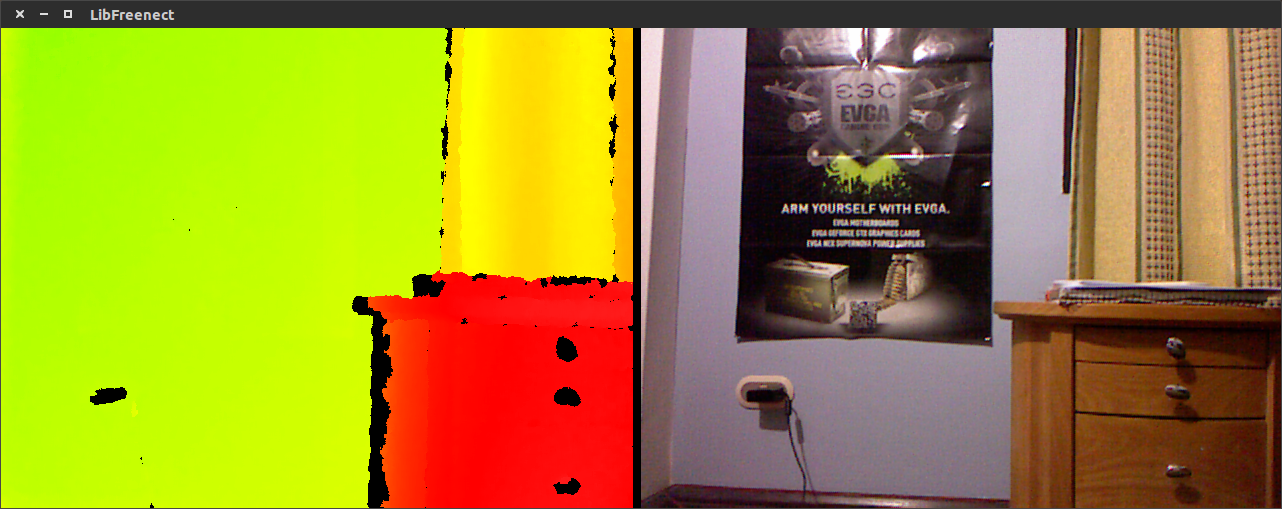
\includegraphics[width=0.75\textwidth]{freenecttest}
\caption{Comprobación de las cámaras del Kinect}
\label{figure:freenecttest}
\end{figure}

Para ello se ha cumplido tanto con la instalación independiente como con la instalación integrada a ROS y se ha comprobado el reconocimiento del Kinect a través del comando:

\begin{blackcodebox}
\begin{lstlisting}[language=bash]
freenect-glview
\end{lstlisting}
\end{blackcodebox}

el cual muestra las imágenes provenientes de ambas cámaras, como se muestra en la figura \ref{figure:freenecttest}

Una vez realizada esta comprobación, podemos continuar con la generación de un mapa de entorno 3D.

\subsubsection{Generación de mapas 3D}

Para esto, realizamos el reconocimiento del entorno a través de la aplicación independiente. Para ello, se inició un terminal y se escribió el comando:

\begin{blackcodebox}
\begin{lstlisting}[language=bash]
rtabmap
\end{lstlisting}
\end{blackcodebox}

cuyo binario está instalado en \url{/usr/local/bin/rtabmap}. Este procedimiento ejecuta el programa, el cual nos pregunta en la primera inicialización, dónde deseamos guardar los datos de la captura (por defecto, esto se realiza en la carpeta \url{/home/<usuario>/Documents/RTAB-Map}).

---Insertar imagen de pregunta---

Tras iniciar, se nos presenta la siguiente pantalla:

---Insertar imagen de pantalla inicial---

Para comenzar la captura de datos de entorno, inicializamos una nueva base de datos haciendo clic en el botón ``New database'':

el cual genera las estructuras de datos necesarias y tras su culminación, estamos listos para realizar la captura. Hacemos clic en el botón Iniciar:

---Insertar imagen de botón iniciar---

Ya podemos comenzar a explorar el entorno. Simplemente basta con dirigir el Kinect haciendo un recorrido del área a obtener, mientras se supervisa la interfaz gráfica de RTAB-Map.

---Insertar imagen de proceso intermedio---

Si en algún momento de la exploración, la pantalla de ``\textit{odometry}'' (odometría) muestra un fondo rojo junto con una imagen estática del entorno, quiere decir que no se tienen suficientes características distintivas en la zona capturada para poder realizar una medición adecuada. Para arreglarlo, tal como se nos indica en el tutorial correspondiente, debemos colocar la cámara de nuevo en la zona que se muestra en la imagen y esperar a que la aplicación retome la generación del mapa desde ese punto.

Una vez explorado el área, hacemos clic en el botón ``Stop'', tras lo cual podemos examinar los resultados, presentados en la figura \ref{figure:bedroommap}.

\begin{figure}[hb]
\centering
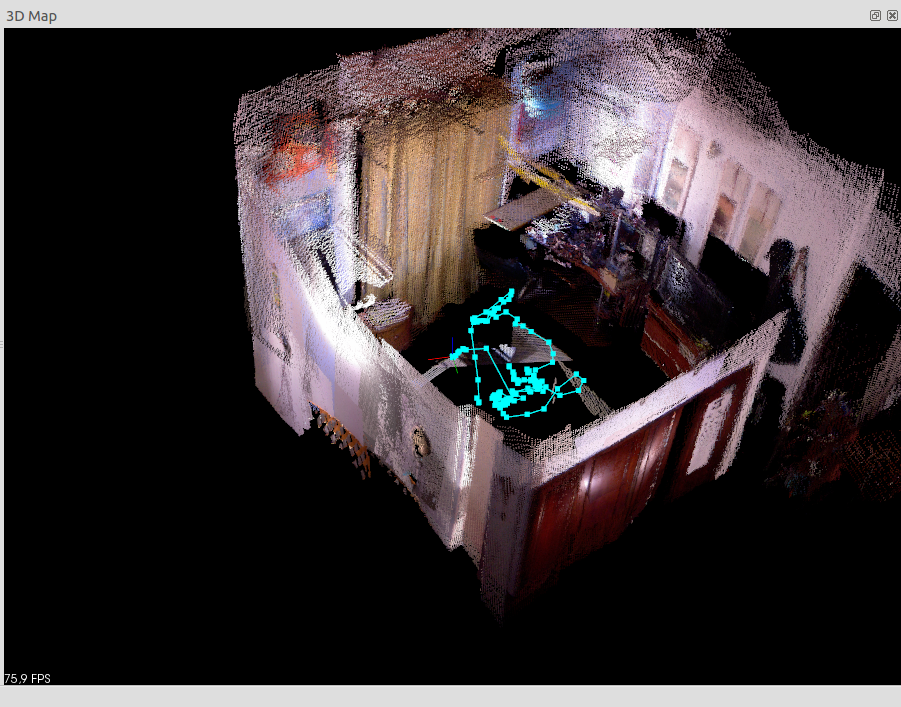
\includegraphics[width=1.00\textwidth]{bedroommap}
\caption{Generación de nube de puntos de una habitación}
\label{figure:bedroommap}
\end{figure}

En el mapa 3D generado, se puede observar una serie de puntos en cian conectados entre sí, que representan la trayectoria de la cámara (en este caso, del Kinect), al generar el mapa.

\subsubsection{Generación de mapas 2D}

La generación de un mapa 2D no es sino la proyección en el plano de la nube de puntos capturada en el paso anterior. Para esto, utilizaremos la versión de RTAB-Map integrada a ROS, ya que por inconvenientes al momento de instalar la versión independiente, no se reconoce de forma adecuada la librería PCL, necesaria para generar la ``rejilla de ocupación'' (en inglés, ``\textit{occupancy grid}'') que sería el mapa en 2D de los obstáculos detectados durante la generación del mapa.

Procedemos de la siguiente forma:

En primer lugar, requeriremos el uso del software de control para el Turtlebot \cite{turtlebot}, que es un kit robótico de bajo costo. Este software permite simular un robot y provee de archivos de lanzamiento adecuados para nuestro caso de uso. Se instala mediante el siguiente comando:

\begin{blackcodebox}
\begin{lstlisting}[language=bash]
sudo apt-get install ros-indigo-turtlebot ros-indigo-turtlebot-apps ros-indigo-turtlebot-interactions ros-indigo-turtlebot-simulator ros-indigo-kobuki-ftdi ros-indigo-rocon-remocon ros-indigo-rocon-qt-library ros-indigo-ar-track-alvar-msgs
\end{lstlisting}
\end{blackcodebox}

Una vez instalado, debemos agregar dos archivos de lanzamiento particulares al directorio de instalación de Turtlebot en ROS, disponibles en el repositorio en Github del proyecto de RTAB-Map en la dirección \url{https://github.com/introlab/rtabmap_ros/}, ejecutando los siguientes comandos en una terminal:

\begin{blackcodebox}
\begin{lstlisting}[language=bash]
sudo wget -P /opt/ros/indigo/share/rtabmap_ros/launch/demo/ https://raw.githubusercontent.com/introlab/rtabmap_ros/master/launch/demo/demo_turtlebot_mapping.launch
sudo wget -P /opt/ros/indigo/share/rtabmap_ros/launch/demo/ https://raw.githubusercontent.com/introlab/rtabmap_ros/master/launch/demo/demo_turtlebot_rviz.launch
\end{lstlisting}
\end{blackcodebox}

Una vez terminadas las descargas, debemos ejecutar cada uno de estos comandos en una terminal independiente:

\begin{blackcodebox}
\begin{lstlisting}[language=bash]

\end{lstlisting}
\end{blackcodebox}

\begin{blackcodebox}
\begin{lstlisting}[language=bash]

\end{lstlisting}
\end{blackcodebox}

\begin{blackcodebox}
\begin{lstlisting}[language=bash]

\end{lstlisting}
\end{blackcodebox}

Este último comando inicia la herramienta RViz, o Visualizador de ROS, el cual permite obtener datos de distintos nodos y tópicos disponibles.

---Insertar imagen de RViz---



---Llenar.---

\paragraph{Selección de altura máxima para generación del mapa 2D}

---Llenar.--- % RTAB-Map y Generación de Mapas

\chapter{Conclusión y Recomendaciones}

\section{Conclusión}

El campo de la robótica es de suma importancia debido a la demanda para realizar tareas repetitivas, peligrosas, de alta precisión, la exploración del terreno, vigilancia, transporte de bienes y personas; todos estos campos y un sinnúmero más cuentan con un creciente soporte gracias a las investigaciones realizadas por universidades y grupos afines, al igual que empresas en el área comercial y militar, lo cual le hace merecedor de más estudio y desarrollo por parte de la Universidad de Los Andes, así como en nuestro país.

Para ello, es preciso entender que el desarrollo de software para robots está orientado al de plataformas de software debido a su capacidad de abstracción, modularización y amplio soporte por parte de comunidades de desarrolladores. Esto lo hace recomendable por encima del desarrollo de aplicaciones personalizadas para cada plataforma de hardware independiente.

Dentro de las plataformas de software consideradas, ROS es la mejor opción por la popularidad que cuenta en la comunidad de investigación y desarrollo robótico, el soporte al desarrollador a cualquier nivel entre novato a experto y la cantidad de módulos existentes para soportar distintos dispositivos o funcionalidades. No obstante, esto no significa que sea la única alternativa disponible, ya que otras plataformas son compatibles con ROS y pueden usarse en paralelo o sustituyéndola por completo.

Por otro lado, para fomentar el desarrollo de robots autónomos utilizando visión por computadora, es factible el uso de Kinect por su bajo costo (en especial al compararlo con sensores de medición láser) y facilidad de uso, a pesar de las limitaciones que pudiera tener, tales como rango y campo de visión limitado y la necesidad de poseer alimentación de corriente adecuada para el uso por parte de un robot móvil.

En lo que respecta al soporte del sistema operativo y de la plataforma de software elegida, contamos con distintos controladores, así como con alternativas de módulos para la generación de mapas de entorno, ya sea de forma individual o en conjunto con sensores láser y codificadores para la odometría. Si bien este proyecto se enfocó en la evaluación de un módulo particular, se tienen otras opciones que podrían proveer de funcionalidades adicionales a las ya exploradas.

La generación del mapa de entorno se realizó mediante la elaboración de nubes de puntos provistas por el Kinect, por lo cual se comprobó su funcionamiento adecuado; de igual forma, se comprobó la coincidencia de la proyección 2D y el mapa de ocupación resultante con la detección de la nube de puntos.

Por último, es menester mencionar la utilidad de la aplicación de las metodologías Ágiles durante el desarrollo de este proyecto; éstas son por definición poco estrictas, en el sentido que permiten tomar o dejar de ellas lo que se requiera o no, por lo cual resultó factible y deseable tomar sencillamente algunos aspectos de cada método utilizado para, tal como el nombre indica, agilizar y facilitar el avance del proyecto sin que la aplicación del o de los métodos se convitiese en una carga adicional para el estudiante o el profesor tutor.

\section{Recomendaciones}

Este proyecto tiene el potencial, si se quiere, de impulsar numerosos desarrollos en LaSDAI para la promoción, desarrollo e implementación de robots móviles autónomos. Por esto, se pueden realizar las siguientes recomendaciones:

\begin{itemize}
	\itemsep1pt \parskip1pt \parsep1pt
	\item Actualizar el sitio web de LaSDAI, incorporando las fuentes a los proyectos realizados y crear un repositorio de código público que los contenga.

	\item Agregar una wiki, accesible públicamente, para colaboración de sus miembros.

	\item Continuar con el desarrollo del proyecto en al menos las siguientes áreas: integración del hardware de un robot móvil en ROS, detección de objetos o personas específicas utilizando OpenNI y Kinect.

	\item Proponer la implementación del desarrollo y control de proyectos en el laboratorio y/o en la escuela de sistemas utilizando Kanban y metodologías Ágiles, llevándolo inclusive al control de flujo de los distintos proyectos de grado dentro de la escuela.
\end{itemize}

% Estilo de la bibliografía
\bibliographystyle{IEEEtranNes}
% Modificada ya que la original está en inglés.

% ***************************************************************** %
% Para agregar toda la bibliografia del archivo .bib
% solo descomente el siguiente comando
% ***************************************************************** %
\nocite{*}

% ***************************************************************** %
% Nombre del archivo con extensión .bib en donde se almacena la bibliografía
\bibliography{Referencias}

% ***************************************************************** %
% FIN DE
% Cuerpo
% ***************************************************************** %

\end{document}
